\documentclass{article}

% =========================================================
% CONFIGURACIÓN GENERAL
% =========================================================

\usepackage[
    letterpaper,
    top=3cm,
    bottom=3cm,
    left=3cm,
    right=3cm,
    headheight=70pt,
    headsep=15pt,
    footskip=30pt,
    includehead
]{geometry}

\usepackage[spanish, es-tabla]{babel}
\spanishdeactivate{"}
\usepackage{csquotes}
\usepackage[utf8]{inputenc}
\usepackage[T1]{fontenc}

% =========================================================
% PAQUETES
% =========================================================

\usepackage{fontawesome5}
\usepackage{amsmath}
\usepackage{amssymb}
\usepackage{graphicx}
\usepackage{stackengine}
\usepackage{fancyhdr}
\usepackage{multicol}
\usepackage{tabularx}
\usepackage{booktabs}
\usepackage{float}
\usepackage{adjustbox}
\usepackage{caption}
\usepackage{xcolor}
\usepackage{listings}
\usepackage{pdflscape}
% \usepackage{microtype} % Desactivado para acelerar compilacion y evitar timeout en Overleaf

% =========================================================
% CONFIGURACIÓN DE LISTINGS
% =========================================================

\lstset{
    basicstyle=\ttfamily\scriptsize,
    backgroundcolor=\color{gray!10},
    keywordstyle=\color{blue}\bfseries,
    stringstyle=\color{teal},
    commentstyle=\color{gray}\itshape,
    frame=single,
    breaklines=true,
    showstringspaces=false,
    tabsize=4,
    captionpos=b
}

% =========================================================
% REFERENCIAS BIBLIOGRÁFICAS
% =========================================================

% =========================================================
% GENERACIÓN AUTOMÁTICA DE BIBLIOGRAFÍA PARA OVERLEAF
% =========================================================

\begin{filecontents*}{\jobname.bib}
@article{cortez2009modeling,
  title={Modeling wine preferences by data mining from physicochemical properties},
  author={Cortez, Paulo and Cerdeira, Ant{\'o}nio and Almeida, Fernando and Matos, Telmo and Reis, Jos{\'e}},
  journal={Decision Support Systems},
  volume={47},
  number={4},
  pages={547--553},
  year={2009},
  publisher={Elsevier}
}

@article{cendrowska1987prism,
  title={{PRISM}: An algorithm for inducing modular rules},
  author={Cendrowska, Jadwiga},
  journal={International Journal of Man-Machine Studies},
  volume={27},
  number={4},
  pages={349--370},
  year={1987},
  publisher={Academic Press}
}


@article{zadeh1965fuzzy,
  title={Fuzzy sets},
  author={Zadeh, Lotfi A},
  journal={Information and Control},
  volume={8},
  number={3},
  pages={338--353},
  year={1965},
  publisher={Elsevier}
}

@article{mamdani1975experiment,
  title={An experiment in linguistic synthesis with a fuzzy logic controller},
  author={Mamdani, Ebrahim H and Assilian, Sedrak},
  journal={International Journal of Man-Machine Studies},
  volume={7},
  number={1},
  pages={1--13},
  year={1975},
  publisher={Elsevier}
}

@book{goldberg1989genetic,
  title={Genetic Algorithms in Search, Optimization, and Machine Learning},
  author={Goldberg, David E},
  year={1989},
  publisher={Addison-Wesley}
}

@book{holland1975adaptation,
  title={Adaptation in Natural and Artificial Systems: An Introductory Analysis with Applications to Biology, Control, and Artificial Intelligence},
  author={Holland, John H},
  year={1975},
  publisher={University of Michigan Press}
}
\end{filecontents*}

\usepackage[
    backend=biber,
    style=ieee,
    sorting=none
]{biblatex}

\addbibresource{\jobname.bib}
\IfFileExists{referencias.bib}{\addbibresource{referencias.bib}}{}

% =========================================================
% HIPERVÍNCULOS
% =========================================================

\usepackage[
    colorlinks=true,
    allcolors=blue
]{hyperref}

% =========================================================
% CONFIGURACIÓN DEL DOCUMENTO
% =========================================================

\newcommand{\checkedbox}{%
    \stackinset{c}{0pt}{c}{0pt}{\checkmark}{$\square$}
}

\pagestyle{fancy}
\fancyhf{}

\setlength{\headheight}{70pt}

% =========================================================
% ENCABEZADO INSTITUCIONAL
% =========================================================

\fancyhead[C]{%
    \begin{minipage}[c]{2.5cm}
        \centering
        \IfFileExists{imagenes/uta.png}{
\includegraphics[width=2.2cm]{imagenes/uta.png}}{\rule{2.2cm}{1.2cm}}
    \end{minipage}%
    \hfill
    \begin{minipage}[c]{8.5cm}
        \centering
        \small{\textbf{UNIVERSIDAD TÉCNICA DE AMBATO}}\\[0.1cm]
        \scriptsize{\textit{FACULTAD DE INGENIERÍA EN SISTEMAS, ELECTRÓNICA E INDUSTRIAL}}\\[0.1cm]
        \scriptsize{\textbf{CARRERA DE SOFTWARE}}\\[0.1cm]
        \scriptsize{\textbf{CICLO ACADÉMICO: JULIO -- DICIEMBRE 2026}}
    \end{minipage}%
    \hfill
    \begin{minipage}[c]{2.5cm}
        \centering
        \IfFileExists{imagenes/fisei.png}{
\includegraphics[width=2.2cm]{imagenes/fisei.png}}{\rule{2.2cm}{1.2cm}}
    \end{minipage}%
}

\fancyfoot[C]{\thepage}

% =========================================================
% CUERPO DEL DOCUMENTO
% =========================================================

\begin{document}

% =========================================================
% PORTADA
% =========================================================

\begin{titlepage}

    \thispagestyle{empty}

    \begin{center}

        \vspace*{0.3cm}

        \IfFileExists{imagenes/uta.png}{%
            
\includegraphics[width=3.8cm]{imagenes/uta.png}%
        }{%
            \rule{3.8cm}{1.8cm}%
        }

        \vspace{0.6cm}

        {\Large \textbf{UNIVERSIDAD TÉCNICA DE AMBATO}}

        \vspace{0.3cm}

        {\large
        FACULTAD DE INGENIERÍA EN SISTEMAS,\\
        ELECTRÓNICA E INDUSTRIAL}

        \vspace{0.4cm}

        {\large \textbf{CARRERA DE SOFTWARE}}

        \vspace{0.6cm}

        {\normalsize
        \textbf{Tema:}\\
        \textbf{SISTEMA INTELIGENTE DE CLASIFICACIÓN DE CALIDAD DEL VINO TINTO MEDIANTE REGLAS PRISM, LÓGICA DIFUSA MAMDANI Y ALGORITMOS GENÉTICOS}

        \vspace{0.3cm}

        \textbf{Unidad de Organización Curricular:}\\
        Profesional

        \vspace{0.3cm}

        \textbf{Nivel y Paralelo:}\\
        7mo -- A

        \vspace{0.3cm}

        \textbf{Asignatura:}\\
        Inteligencia Artificial

        \vspace{0.3cm}

        \textbf{Docente:}\\
        Ing. Mg. Ruben Nogales

        \vspace{0.3cm}

        \textbf{Alumnos participantes:}\\
        Toala Steeven\\
        Chavez Michael

        }

        \vfill

        {\normalsize
        Ambato -- Ecuador\\
        Septiembre de 2026
        }

    \end{center}

\end{titlepage}

% =========================================================
% ÍNDICES
% =========================================================

\pagenumbering{roman}

\tableofcontents
\newpage

\listoffigures
\newpage

\listoftables
\newpage

\pagenumbering{arabic}

% =========================================================
% 1. DEFINICIÓN DEL PROBLEMA
% =========================================================

\section{Definición del Problema}

\subsection{Contexto Enológico y Descripción del Dataset}

El control de calidad enológico constituye un proceso crítico en la industria vitivinícola global. La evaluación organoléptica tradicional del vino depende de comités de cata sensorial certificados. Si bien la cata humana aporta una valoración holística insustituible, está condicionada por factores subjetivos inevitables: fatiga sensorial del paladar tras múltiples muestras, sesgos de percepción individual, oscilaciones de temperatura ambiente y elevados costes logísticos y temporales por sesión de catado. Por estas razones, el modelado computacional y la caracterización analítica mediante técnicas de Inteligencia Artificial (IA) representan un soporte objetivo de alto valor para enólogos y bodegueros \cite{cortez2009modeling}.

El presente estudio utiliza el conjunto de datos de referencia \textit{Wine Quality Dataset} (variante de vino tinto \textit{Vinho Verde}), publicado por Cortez et al. \cite{cortez2009modeling} y alojado en el repositorio de Machine Learning de la Universidad de California en Irvine (UCI). El conjunto consta de $N = 1,599$ muestras fisicoquímicas reales de vino tinto, analizadas exhaustivamente mediante 11 variables continuas obtenidas por espectrometría y química analítica, junto con una variable objetivo sensorial denominada \texttt{quality}, correspondiente a la mediana de las calificaciones otorgadas por al menos tres catadores expertos en una escala ordinal de 0 a 10.

\subsection{El Dilema de Caja Negra vs. El Problema de Frontera}

Al abordar la predicción de la calidad sensorial del vino mediante sistemas computacionales surgen dos vertientes clásicas en la literatura, ambas aquejadas de limitaciones estructurales:
\begin{enumerate}
    \item \textbf{Modelos de Caja Negra (\textit{Black-Box}):} Métodos avanzados como Redes Neuronales Artificiales profundas (ANN), Máquinas de Soporte Vectorial (SVM) o Ensambles de Árboles (XGBoost) logran un ajuste numérico aceptable, pero carecen por completo de transparencia y trazabilidad en sus decisiones internas. Si un lote de producción es calificado como defectuoso o subestándar, el enólogo no puede deducir la causalidad físico-química que originó dicha clasificación, imposibilitando la intervención correctiva en las etapas de fermentación, maceración o crianza en bodega \cite{cortez2009modeling}.
    \item \textbf{Modelos Basados en Reglas Clásicas Booleanas:} Los clasificadores de reglas simbólicas discretas ($SI \dots ENTONCES \dots$) ofrecen máxima interpretabilidad, pero sufren de manera severa del denominado \textbf{problema de frontera} (\textit{boundary problem}). Si una regla booleana establece como condición $\text{Alcohol} > 10.80\%$, un vino de características excepcionales que presente un tenor alcohólico de $10.79\%$ es rechazado con la misma rigidez que una muestra deficiente con $8.50\%$. Esta discontinuidad binaria provoca caídas masivas en la cobertura de muestras (abstención de clasificación ante patrones no contemplados con exactitud) y una extrema vulnerabilidad ante el ruido analítico de medición de laboratorio.
\end{enumerate}

Para resolver esta dicotomía sin sacrificar la interpretabilidad se formula una \textbf{arquitectura secuencial e híbrida} estructurada en cuatro fases fundamentales:
\begin{enumerate}
    \item \textbf{Fase 1: Preparación y Análisis Químico:} Ingesta de datos, validación univariada de las 11 variables fisicoquímicas continuas, matriz de correlación de Pearson y partición estratificada $80/20$ con discretización balanceada por terciles.
    \item \textbf{Fase 2: Inducción Modular de Reglas con PRISM:} Extracción de reglas de clasificación directas mediante recubrimiento secuencial (\textit{separate-and-conquer}) formulado por Cendrowska \cite{cendrowska1987prism}, evidenciando las limitaciones del clasificador rígido ante el problema de frontera.
    \item \textbf{Fase 3: Inferencia Difusa Continua Mamdani:} Suavizado continuo de las fronteras mediante conjuntos difusos \cite{zadeh1965fuzzy}, funciones de pertenencia continuas híbridas (Trapezoidales en hombros y Triangulares en el centro), implicación con T-norma Gödel ($\min$), agregación S-norma ($\max$) y defuzzificación por Centroide de Gravedad (CoG) \cite{mamdani1975experiment}.
    \item \textbf{Fase 4: Calibración Evolutiva con Algoritmo Genético:} Sintonización simultánea de los puntos de corte difusos y factores de ponderación de las reglas mediante computación evolutiva basada en Holland \cite{holland1975adaptation} y Goldberg \cite{goldberg1989genetic}, desarrollada íntegramente desde cero sin cajas negras.
\end{enumerate}

\subsection{Justificación Bioquímica y Conservación de las 11 Variables}

A diferencia de aproximaciones reduccionistas que descartan arbitrariamente variables hasta trabajar con solo 4 propiedades, este proyecto defiende la \textbf{conservación integral de las 11 variables fisicoquímicas continuas}. En enología, la calidad sensorial es una propiedad emergente producto del balance molecular; prescindir de variables secundarias genera <<puntos ciegos>> analíticos que impiden detectar defectos de conservación o desviaciones fermentativas. La Tabla \ref{tab:variables_quimicas} detalla el rango empírico de cada propiedad en el dataset y su justificación bioquímica.

\begin{table}[H]
\centering
\caption{Variables fisicoquímicas continuas del vino tinto y su función enológica.}
\label{tab:variables_quimicas}
\small
\begin{tabularx}{\textwidth}{p{3.2cm}ccX}
\toprule
\textbf{Variable Fisicoquímica} & \textbf{Unidad} & \textbf{Rango Empírico} & \textbf{Rol Bioquímico y Sensorial en el Vino Tinto} \\
\midrule
\textit{Fixed Acidity} (Acidez Fija) & $\text{g/dm}^3$ & $[4.60, 15.90]$ & Ácidos orgánicos no volátiles (tartárico, málico). Confiere soporte estructural, frescura y viveza inicial en boca. \\
\textit{Volatile Acidity} (Acidez Volátil) & $\text{g/dm}^3$ & $[0.12, 1.58]$ & Ácido acético producido por bacterias acéticas. Biomarcador primario de deterioro (\textit{vinagrado}). Niveles altos arruinan el vino. \\
\textit{Citric Acid} (Ácido Cítrico) & $\text{g/dm}^3$ & $[0.00, 1.00]$ & Aporta frescura cítrica y actúa como quelante natural de cationes de hierro y cobre, previniendo quiebras férricas. \\
\textit{Residual Sugar} (Azúcar Residual) & $\text{g/dm}^3$ & $[0.90, 15.50]$ & Glucosa y fructosa no fermentadas. En vinos secos ($<3.0\,\text{g/dm}^3$), suaviza la astringencia de taninos y alcohol. \\
\textit{Chlorides} (Cloruros) & $\text{g/dm}^3$ & $[0.012, 0.611]$ & Sales minerales disueltas (NaCl). Modulan la salinidad y untuosidad; concentraciones excesivas confieren sabor salino defectuoso. \\
\textit{Free Sulfur Dioxide} ($\text{SO}_2$ Libre) & $\text{mg/dm}^3$ & $[1.0, 72.0]$ & Fracción activa de dióxido de azufre molecular. Agente antimicrobiano y antioxidante indispensable para prevenir la oxidación. \\
\textit{Total Sulfur Dioxide} ($\text{SO}_2$ Total) & $\text{mg/dm}^3$ & $[6.0, 289.0]$ & Suma de fracciones libres y ligadas. Su exceso enmascara aromas frutales y produce notas picantes indeseables. \\
\textit{Density} (Densidad) & $\text{g/cm}^3$ & $[0.990, 1.004]$ & Vinculada al extracto seco libre y grado alcohólico. Refleja la concentración y densidad de cuerpo del caldo. \\
\textit{pH} & Unidades & $[2.74, 4.01]$ & Concentración $[\text{H}^+]$. Regula la eficacia del $\text{SO}_2$, estabilidad microbiana y la intensidad de color antociánico. \\
\textit{Sulphates} (Sulfatos) & $\text{g/dm}^3$ & $[0.33, 2.00]$ & Aditivo enológico ($\text{K}_2\text{SO}_4$) que promueve la formación de $\text{SO}_2$ libre y preserva el perfil aromático frutal. \\
\textit{Alcohol} & \% vol & $[8.40, 14.90]$ & Etanol fermentativo. Variable con mayor correlación univariada ($r \approx 0.48$) con la calidad percibida y calidez en boca. \\
\bottomrule
\end{tabularx}
\end{table}

\subsection{Categorización de la Variable Objetivo y Desbalance de Clases}

Las notas sensoriales originales en la escala $[3, 8]$ fueron agregadas en 3 categorías cualitativas representativas del estándar enológico internacional:
\begin{itemize}
    \item \textbf{Calidad Baja (notas 3, 4 y 5):} 744 muestras ($46.53\%$). Vinos desequilibrados, con acidez volátil excesiva o aromas apagados.
    \item \textbf{Calidad Media (nota 6):} 638 muestras ($39.90\%$). Vinos comerciales estándar de consumo masivo con correcto balance general.
    \item \textbf{Calidad Alta (notas 7 y 8):} 217 muestras ($13.57\%$). Vinos excepcionales, reserva o gran reserva, con perfil armónico sobresaliente.
\end{itemize}

El marcado desbalance entre la clase minoritaria \textit{Alta} ($13.57\%$) y las clases mayoritarias ($86.43\%$ acumulado) plantea un reto de modelado: una función de optimización ingenua basada en exactitud global (\textit{Accuracy}) colapsaría prediciendo únicamente clases mayoritarias, ignorando los vinos de alta gama. Este desafío se resuelve mediante la formulación de una función de aptitud multi-criterio en el Algoritmo Genético.

% =========================================================
% 2. MEDIDAS DE EVALUACIÓN DE REGLAS
% =========================================================

\section{Medidas de Evaluación de Reglas}

\subsection{Métricas Inductivas de Clasificación (PRISM)}

El algoritmo PRISM \cite{cendrowska1987prism} utiliza una heurística voraz para extraer reglas modulares de la forma $SI \; Antecedente \; ENTONCES \; Consecuente$. Las métricas fundamentales que rigen su funcionamiento son:

\begin{enumerate}
    \item \textbf{Precisión Condicional (Pureza de la Regla):} Dado un subconjunto de instancias $S$ cubiertas por un antecedente candidato y la clase objetivo $C_j$, se define:
    \begin{equation}
        p/t = \frac{|S \cap C_j|}{|S|}
    \end{equation}
    donde $p$ es la cantidad de instancias en $S$ que pertenecen efectivamente a la clase $C_j$, y $t = |S|$ es el total de instancias cubiertas por la condición. PRISM maximiza $p/t$ en cada paso iterativo.
    \item \textbf{Cobertura de Regla:} Proporción de instancias del conjunto total de entrenamiento que satisfacen el antecedente de la regla:
    \begin{equation}
        \text{Cobertura}(R) = \frac{|S|}{N_{\text{total}}}
    \end{equation}
    Una vez que una regla alcanza la pureza requerida (e.g. $p/t \ge 0.65$), las $p$ instancias cubiertas correctamente son removidas del conjunto de entrenamiento mediante el principio de \textbf{recubrimiento secuencial} (\textit{separate-and-conquer}), permitiendo inducir reglas especializadas para las instancias residuales.
\end{enumerate}

\subsection{Métricas de Evaluación de Reglas en PRISM (Confianza, Soporte, Cobertura y Lift)}

En la implementación del algoritmo PRISM (\texttt{Fase\_2\_PRISM/prism.py}), cada regla modular candidata no solo es evaluada por su pureza condicional inmediata, sino que se calculan formalmente cuatro métricas probabilísticas y estadísticas de calidad para cuantificar su representatividad enológica:

\begin{enumerate}
    \item \textbf{Confianza o Precisión de la Regla (\textit{Confidence}):} Probabilidad condicional de que un vino pertenezca a la clase consecuente $C_j$ dado que satisface las restricciones del antecedente $A$:
    \begin{equation}
        \text{Confianza}(A \to C_j) = P(C_j \mid A) = \frac{|\sigma(A \cup C_j)|}{|\sigma(A)|}
    \end{equation}
    donde $|\sigma(A)|$ representa la cantidad de instancias que cumplen las condiciones fisicoquímicas y $|\sigma(A \cup C_j)|$ las que además pertenecen a la clase evaluada.
    \item \textbf{Soporte (\textit{Support}):} Proporción de vinos del conjunto total de entrenamiento que cumplen simultáneamente el antecedente y el consecuente de la regla:
    \begin{equation}
        \text{Soporte}(A \to C_j) = P(A \cup C_j) = \frac{|\sigma(A \cup C_j)|}{N_{\text{total}}}
    \end{equation}
    \item \textbf{Cobertura de Clase (\textit{Coverage}):} Proporción de muestras positivas de la clase $C_j$ que son explicadas por la regla:
    \begin{equation}
        \text{Cobertura}(A \to C_j) = \frac{|\sigma(A \cup C_j)|}{|\sigma(C_j)|}
    \end{equation}
    \item \textbf{Sustentación o Elevación (\textit{Lift}):} Razón de correlación estadística entre la regla y la probabilidad previa independiente $P(C_j)$ de la clase en el lote de entrenamiento:
    \begin{equation}
        \text{Lift}(A \to C_j) = \frac{\text{Confianza}(A \to C_j)}{P(C_j)} = \frac{P(A \cup C_j)}{P(A) \cdot P(C_j)}
    \end{equation}
    Un valor de $\text{Lift} > 1.0$ certifica que la combinación de características fisicoquímicas seleccionada multiplica la probabilidad de pertenencia a dicha categoría en comparación con el azar. En el entrenamiento de \texttt{Proyecto\_Calidad\_Vino}, el algoritmo descubrió reglas con $\text{Lift}$ de hasta $\mathbf{5.05}$ para la clase minoritaria crítica (\textit{ALTA}).
\end{enumerate}

\subsection{Métricas Globales de Desempeño del Clasificador}

Para evaluar rigurosamente el sistema a lo largo de las distintas fases se emplean las siguientes métricas canónicas:
\begin{itemize}
    \item \textbf{Exactitud (\textit{Accuracy}):} Fracción de clasificaciones correctas sobre el total de muestras:
    \begin{equation}
        \text{Accuracy} = \frac{\sum_{c} TP_c}{N}
    \end{equation}
    \item \textbf{Recall por Clase y F1-Macro:} Dado el fuerte desbalance de clases ($46.5\%$ Baja, $39.9\%$ Media y solo $13.6\%$ Alta), el promedio macro de F1 es la métrica de convergencia principal:
    \begin{equation}
        \text{Recall}_c = \frac{TP_c}{TP_c + FN_c}, \quad \text{Precision}_c = \frac{TP_c}{TP_c + FP_c}
    \end{equation}
    \begin{equation}
        F_{1,\text{macro}} = \frac{1}{|C|} \sum_{c \in C} 2 \cdot \frac{\text{Precision}_c \cdot \text{Recall}_c}{\text{Precision}_c + \text{Recall}_c}
    \end{equation}
    \item \textbf{Cobertura del Sistema:} Porcentaje de muestras para las cuales el sistema activa al menos una regla difusa o booleana, sin incurrir en abstención:
    \begin{equation}
        \text{Cobertura} = \frac{N_{\text{clasificadas}}}{N_{\text{total}}} \times 100\%
    \end{equation}
    \item \textbf{Razón de Parsimonia / Complejidad:} Razón entre reglas activas no redundantes y el total de la base:
    \begin{equation}
        \text{Complejidad} = \frac{N_{\text{activas}}}{N_{\text{totales}}}
    \end{equation}
\end{itemize}

% =========================================================
% 3. FUNDAMENTACIÓN TEÓRICA DE LOS PARADIGMAS DE IA
% =========================================================

\section{Fundamentación Teórica de los Paradigmas de Inteligencia Artificial}

\subsection{Inducción Modular de Reglas Supervisadas (PRISM de Cendrowska)}

El algoritmo PRISM \cite{cendrowska1987prism} representa uno de los hitos fundacionales del aprendizaje inductivo simbólico supervisado. A diferencia de los clasificadores basados en árboles de decisión clásicos (como ID3 o C4.5), que imponen una jerarquía arbórea descendente rígida donde una variable dividida en la raíz fragmenta forzosamente todo el espacio subsecuente, PRISM induce cada regla de manera completamente modular e independiente.

Los árboles de decisión adolecen del denominado \textbf{problema del subárbol replicado} (\textit{replicated subtree problem}): si dos ramas distintas requieren probar la misma condición sobre un atributo químico secundario (por ejemplo, el contenido de sulfatos), el árbol se ve forzado a duplicar subestructuras enteras, diluyendo la muestra estadística en las hojas inferiores. PRISM soluciona esta patología mediante la estrategia de \textbf{recubrimiento secuencial} (\textit{separate-and-conquer}):
\begin{enumerate}
    \item Itera clase por clase de forma supervisada, enfocándose directamente en el objetivo.
    \item Agrega condiciones antecedentes de forma voraz maximizando la probabilidad condicional $p/t$.
    \item Una vez que la regla alcanza la pureza mínima requerida, remueve únicamente los ejemplos positivos cubiertos de esa clase y reinicia el proceso para las instancias restantes.
\end{enumerate}

En \texttt{Proyecto\_Calidad\_Vino}, PRISM induce un conjunto estructurado de \textbf{64 reglas modulares} sobre las 11 variables continuas discretizadas por terciles empíricos, distribuidas balanceadamente entre las tres categorías: 14 reglas especializadas para la clase \textit{ALTA}, 16 reglas para la clase \textit{BAJA} y 34 reglas para la clase \textit{MEDIA}.

\subsection{El Problema de Frontera (Boundary Problem) en Clasificadores Rígidos}

Al evaluar las 64 reglas inducidas mediante una lógica booleana discreta tradicional (\textit{crisp evaluation}), surge el colapso del \textbf{problema de frontera}:
\begin{itemize}
    \item Las particiones discretas establecen umbrales abruptos (e.g. $\text{Alcohol} > 10.8\%$). Una muestra con $10.79\%$ de alcohol es rechazada con la misma severidad binaria que una con $8.5\%$.
    \item Al evaluar en el conjunto de prueba independiente ($N=320$), el modelo rígido obtiene una exactitud de apenas \textbf{33.12\%} (y 35.5\% en entrenamiento), provocando caídas masivas de concordancia y un elevado índice de abstención ante patrones continuos reales no contemplados con rigidez idéntica en el entrenamiento.
\end{itemize}

\subsection{Inferencia Difusa Mamdani: Puente Continuo hacia la Cobertura Total}

Para erradicar la discontinuidad booleana sin perder la transparencia simbólica de las reglas, se introduce la \textbf{Lógica Difusa de Mamdani} \cite{zadeh1965fuzzy, mamdani1975experiment}:
\begin{itemize}
    \item Se sustituyen las fronteras rectangulares por \textbf{funciones de pertenencia continuas} $\mu(x) \in [0, 1]$ (trapezoidales en los extremos para saturación y triangulares en el centro).
    \item Una muestra química no pertenece rígidamente a una única etiqueta, sino que activa simultáneamente múltiples conjuntos lingüísticos con grados de certeza graduales.
    \item Mediante la T-norma de Gödel ($\min$), la agregación por S-norma ($\max$) y la defuzzificación por Centroide de Gravedad (CoG), la cobertura del clasificador alcanza instantáneamente el \textbf{100.0\%} y la exactitud en prueba salta del $33.12\%$ a un contundente \textbf{60.31\%} (+27.19 puntos porcentuales de ganancia directa).
\end{itemize}

\subsection{Computación Evolutiva con Algoritmos Genéticos (John Holland)}

El modelado difuso introduce 33 puntos de corte continuos y 64 factores de ponderación de reglas. Encontrar manualmente la combinación óptima en un espacio no convexo de $59+$ dimensiones continuas es matemáticamente intratable mediante descenso por gradiente convencional debido a la naturaleza no diferenciable de los operadores $\min$ y $\max$.

El \textbf{Algoritmo Genético} de John H. Holland \cite{holland1975adaptation} y David E. Goldberg \cite{goldberg1989genetic} proporciona el mecanismo idóneo de optimización global estocástica. Implementado íntegramente desde cero en Python y NumPy, el algoritmo simula la selección natural mediante torneo, cruce continuo y mutación con reparación de coherencia física, convergiendo en apenas 15.1 segundos hacia una configuración que eleva la exactitud al \textbf{64.82\%} en entrenamiento y \textbf{60.94\%} en prueba, protegiendo activamente la clase minoritaria \textit{ALTA}.

% =========================================================
% 4. IMPLEMENTACIÓN DE LOS ALGORITMOS
% =========================================================

\section{Implementación de los Algoritmos}

\subsection{Arquitectura Modular del Proyecto}

El proyecto se estructuró bajo estándares de ingeniería de software limpios, legibles y rigurosamente desacoplados (PEP 8) en la raíz de \texttt{Proyecto\_Calidad\_Vino}, organizándose en módulos funcionales por fases de Inteligencia Artificial:

\begin{itemize}
    \item \texttt{Fase\_1\_Datos/preparacion.py}: Ingesta del archivo fisicoquímico \texttt{winequality-red.csv}, verificación de integridad (1,599 registros continuos sin valores nulos), cálculo de estadísticas descriptivas univariadas, matriz de correlación de Pearson y discretización no sesgada por terciles empíricos ($33\%$) con partición estratificada $80/20$ ($N_{\text{train}} = 1,279$, $N_{\text{test}} = 320$).
    \item \texttt{Fase\_2\_PRISM/prism.py}: Implementación canónica desde cero del algoritmo PRISM (\textit{separate-and-conquer}) formulado por Cendrowska \cite{cendrowska1987prism}. Inducción modular de reglas supervisadas guiada paso a paso por pureza condicional $p/t$, con cálculo formal de soporte, confianza, sustentación (\textit{Lift}) y exportación de reglas modulares.
    \item \texttt{Fase\_3\_Logica\_Difusa/difuso.py}: Motor de inferencia difusa Mamdani continuo vectorizado en NumPy, estructurado de forma pedagógica y modular en 6 bloques académicos:
    \begin{enumerate}
        \item \textit{Funciones de Pertenencia}: Geometría trapezoidal en los hombros de saturación y triangular en la zona central para las 11 variables continuas.
        \item \textit{Fuzzificación}: Mapeo continuo no lineal de variables fisicoquímicas a grados de membresía lingüísticos.
        \item \textit{Inferencia Mamdani}: Evaluación de antecedentes mediante la T-norma de Gödel ($\min$) ponderada por factores de modulación.
        \item \textit{Agregación Difusa}: Unificación de áreas de corte consecuentes mediante la S-norma de Zadeh ($\max$).
        \item \textit{Defuzzificación CoG}: Integración numérica continua del Centroide de Gravedad sobre el universo $[0, 10]$.
        \item \textit{Funciones de Cálculo}: Mapeo a las tres clases enológicas (\textit{Baja}, \textit{Media}, \textit{Alta}).
    \end{enumerate}
    \item \texttt{Fase\_4\_Algoritmo\_Genetico/genetico.py}: Algoritmo Genético continuo canónico desarrollado íntegramente desde cero según los fundamentos de Holland \cite{holland1975adaptation} y Goldberg \cite{goldberg1989genetic}, prescindiendo deliberadamente de librerías de caja negra (sin dependencias opacas como DEAP). Integra representación de genotipo mixto continuo (puntos de corte de MFs y ponderación de reglas), operador de reparación de coherencia física ($a < b < c$), mecanismos de selección por torneo y ruleta estocástica, cruce continuo, mutación gaussiana acotada, elitismo estricto del top 5\% y convergencia acelerada (11--14 segundos).
    \item \texttt{modelo.py}: Fachada unificada (\textit{Facade Pattern}) que encapsula el pipeline completo de inferencia y expone una API limpia para la predicción y evaluación comparativa.
    \item \texttt{interfaz.py}: Aplicación de escritorio nativa desarrollada en Python con la biblioteca gráfica \textbf{Tkinter} y gráficos interactivos embebidos de \textbf{Matplotlib}. Ofrece un entorno integral de laboratorio con 5 pestañas científicas: Exploración de Datos, Extracción PRISM, Superficie Difusa 3D Mamdani, Convergencia del Algoritmo Genético y Clasificador Enológico en Tiempo Real con visualización continua del CoG.
    \item \texttt{main.py}: Orquestador principal del proyecto que permite la ejecución secuencial completa desde consola o el inicio del entorno gráfico interactivo.
\end{itemize}

\subsection{Sistema de Inferencia Difusa Mamdani Continuo}

Para superar el problema de frontera de las reglas discretas se diseñó un motor de inferencia difusa continuo basado en el modelo de Mamdani \cite{mamdani1975experiment}:

\subsubsection{Funciones de Pertenencia Continuas Híbridas}
Para cada variable química continua $x_i$ ($i = 1, \dots, 11$), se definen tres conjuntos difusos lingüísticos: $\text{Bajo}$, $\text{Medio}$ y $\text{Alto}$, parametrizados por tres puntos de corte ordenados $a_i < b_i < c_i$. Se seleccionó una geometría \textbf{híbrida trapezoidal-triangular}:
\begin{itemize}
    \item \textbf{Conjunto <<Bajo>> (Trapezoide abierto a la izquierda):}
    \begin{equation}
        \mu_{\text{Bajo}}(x_i; a_i, b_i) = \begin{cases}
            1.0, & x_i \le a_i \\
            \frac{b_i - x_i}{b_i - a_i}, & a_i < x_i \le b_i \\
            0.0, & x_i > b_i
        \end{cases}
    \end{equation}
    \item \textbf{Conjunto <<Medio>> (Triángulo simétrico central):}
    \begin{equation}
        \mu_{\text{Medio}}(x_i; a_i, b_i, c_i) = \begin{cases}
            \frac{x_i - a_i}{b_i - a_i}, & a_i < x_i \le b_i \\
            \frac{c_i - x_i}{c_i - b_i}, & b_i < x_i \le c_i \\
            0.0, & \text{en otro caso}
        \end{cases}
    \end{equation}
    \item \textbf{Conjunto <<Alto>> (Trapezoide abierto a la derecha):}
    \begin{equation}
        \mu_{\text{Alto}}(x_i; b_i, c_i) = \begin{cases}
            0.0, & x_i \le b_i \\
            \frac{x_i - b_i}{c_i - b_i}, & b_i < x_i \le c_i \\
            1.0, & x_i > c_i
        \end{cases}
    \end{equation}
\end{itemize}

\textbf{Justificación de la Elección de MFs Lineales a Trozos:}
\begin{enumerate}
    \item \textit{Saturación de Hombros Abiertos:} En variables químicas como el tenor alcohólico o la concentración de sulfitos, los extremos no deben sufrir atenuación de membresía. Un vino con $14.5\%$ de alcohol posee una certeza plena ($\mu = 1.0$) de pertenecer a la clase <<Alto>>, idéntica a una muestra con $13.5\%$. Las campanas gaussianas o curvas sigmoides atenuarían artificialmente los valores ultraaltos.
    \item \textit{Eficiencia Computacional Analítica:} Las funciones lineales a trozos permiten calcular el Centroide de Gravedad analíticamente mediante cálculo diferencial por trapecios en $\approx 2.4\,\text{ms}$ por muestra. Esto fue determinante para que el Algoritmo Genético pudiera evaluar $1,500$ soluciones candidatas en tiempo razonable sin incurrir en cuellos de botella de funciones exponenciales trascendentes.
\end{enumerate}

\subsubsection{Mecanismo de Inferencia, Agregación y Defuzzificación}
Dada una muestra $x \in \mathbb{R}^{11}$, cada regla $R_k$ con peso de modulación $w_k \in [0, 1]$ calcula su grado de activación $\alpha_k$ mediante la T-norma de Gödel ($\min$):
\begin{equation}
    \alpha_k = w_k \cdot \min_{(v, l) \in \text{Antecedentes}(R_k)} \mu_{v, l}(x_v)
\end{equation}

El universo de discurso de la salida difusa se establece en la escala continua de calidad $y \in [0, 10]$, definiendo tres funciones de salida: $\mu_{\text{Baja}}(y) = \text{trapmf}(y; [0, 0, 3.5, 5.0])$, $\mu_{\text{Media}}(y) = \text{trimf}(y; [4.5, 6.0, 7.5])$ y $\mu_{\text{Alta}}(y) = \text{trapmf}(y; [7.0, 8.5, 10, 10])$. La agregación difusa global aplica la S-norma ($\max$):
\begin{equation}
    \mu_{\text{agregada}}(y) = \max_{k=1}^{64} \min\left(\alpha_k, \mu_{\text{Consecuente}(R_k)}(y)\right)
\end{equation}

El valor cuantitativo de calidad continua se obtiene por el método del Centroide de Gravedad (CoG):
\begin{equation}
    y^* = \frac{\int_{0}^{10} y \cdot \mu_{\text{agregada}}(y)\,dy}{\int_{0}^{10} \mu_{\text{agregada}}(y)\,dy}
\end{equation}

La asignación de la clase lingüística final se determina mediante umbrales enológicos calibrados:
\begin{equation}
    \text{Clase}(y^*) = \begin{cases}
        \text{Baja}, & y^* < 5.30 \\
        \text{Media}, & 5.30 \le y^* < 6.60 \\
        \text{Alta}, & y^* \ge 6.60
    \end{cases}
\end{equation}

\subsection{Calibración Evolutiva con Algoritmos Genéticos}

El ajuste manual de las funciones de pertenencia y de los factores de ponderación de las 64 reglas inducidas por PRISM resulta impracticable debido a la alta no linealidad y dimensionalidad del espacio de búsqueda. Por ello, se diseñó e implementó de forma canónica desde cero un Algoritmo Genético continuo basado en los principios fundacionales de Holland \cite{holland1975adaptation} y Goldberg \cite{goldberg1989genetic}, prescindiendo conscientemente de librerías de caja negra (como DEAP) para garantizar la total transparencia y control algorítmico sobre cada operador genético:

\subsubsection{Estructura del Cromosoma Mixto Continuo (97 Genes)}
El genotipo de cada individuo en \texttt{genetico.py} se compone de un vector continuo de parámetros reales:
\begin{itemize}
    \item \textbf{Bloque 1 (33 genes reales):} Puntos de corte de las funciones de pertenencia continuas ($a_i < b_i < c_i$) para cada una de las 11 variables fisicoquímicas continuas.
    \item \textbf{Bloque 2 (64 genes reales en $[0.0, 1.5]$):} Factores de modulación y ponderación para cada una de las 64 reglas modulares de PRISM.
\end{itemize}

\subsubsection{Operador de Reparación y Factibilidad Física}
Para garantizar que las funciones de pertenencia mantengan coherencia semántica en todo momento, se implementó un operador de reparación geométrico estricto que ordena forzosamente los genes tras las operaciones de cruce y mutación:
\begin{equation}
    \min(x_i) \le a_i < b_i < c_i \le \max(x_i) \quad \forall i \in \{1, \dots, 11\}
\end{equation}

\subsubsection{Función de Aptitud y Optimización de la Exactitud}
La función de aptitud evalúa el porcentaje de concordancia predictiva del sistema difuso sobre el conjunto de entrenamiento ($N_{\text{train}} = 1,279$) al evaluar simultáneamente las 64 reglas ponderadas y los cortes continuos actualizados:
\begin{equation}
    \text{Fitness} = \left( \frac{1}{N_{\text{train}}} \sum_{i=1}^{N_{\text{train}}} \mathbb{I}\left( \hat{y}_i = y_i \right) \right) \times 100\%
\end{equation}
donde $\mathbb{I}$ es la función indicadora de acierto y la predicción $\hat{y}_i$ se obtiene evaluando vectorialmente las activaciones ponderadas $\alpha_k \cdot w_k$ acumuladas hacia cada clase consecuente (\textit{ALTA}, \textit{MEDIA}, \textit{BAJA}).

La Tabla \ref{tab:hiperparametros_ga} detalla los hiperparámetros evolutivos exactos programados en \texttt{Fase\_4\_Algoritmo\_Genetico/genetico.py}.

\begin{table}[H]
\centering
\caption{Hiperparámetros de calibración del Algoritmo Genético en \texttt{genetico.py}.}
\label{tab:hiperparametros_ga}
\small
\begin{tabularx}{\textwidth}{p{4.2cm}p{3.6cm}X}
\toprule
\textbf{Hiperparámetro} & \textbf{Valor Programado} & \textbf{Justificación Técnica y Fundamento} \\
\midrule
Tamaño de Población & 25 individuos & Eficiencia computacional y diversidad balanceada en espacio continuo. \\
Número de Generaciones & 25 épocas & Suficiente para estabilizar la meseta de convergencia sin sobreajuste. \\
Probabilidad de Cruce ($P_c$) & 0.85 (85.0\%) & Fomenta recombinación genética activa de bloques constructores. \\
Tipo de Cruce & Cruce Aritmético y 1 Punto & Recombinación continua de cortes difusos y vectores de pesos. \\
Probabilidad de Mutación ($P_m$) & 0.20 (20.0\%) & Exploración estocástica controlada evitando óptimos locales prematuros. \\
Tipo de Mutación & Variación acotada con clip & Perturbación uniforme dentro del 8\% del rango físico de cada variable. \\
Mecanismo de Selección & Torneo ($k=3$) / Ruleta & Presión selectiva equilibrada que favorece a los individuos más aptos. \\
Elitismo & 2 individuos élite & Preservación estricta de las mejores soluciones sin degradación generacional. \\
Tiempo de Ejecución & $\approx 15.10$ segundos & Convergencia ultrarrápida vectorizada en NumPy nativo. \\
\bottomrule
\end{tabularx}
\end{table}

% =========================================================
% 5. CASOS DE PRUEBA Y RESULTADOS EXPERIMENTALES
% =========================================================

\section{Casos de Prueba y Resultados Experimentales}

\subsection{Protocolo Experimental y División de Datos}

El dataset de 1,599 muestras se dividió mediante muestreo estratificado no sesgado en un $80\%$ para entrenamiento ($N_{\text{train}} = 1,279$) y un $20\%$ para prueba independiente ($N_{\text{test}} = 320$), fijando la semilla aleatoria en 42 para garantizar plena reproducibilidad.

\subsection{Benchmarking Progresivo a Través de las Fases del Proyecto}

La Tabla \ref{tab:benchmarking_fases} presenta la comparativa formal de desempeño en el conjunto de entrenamiento ($N_{\text{train}}=1,279$) y en el conjunto ciego de prueba ($N_{\text{test}}=320$) a través de las etapas metodológicas implementadas en \texttt{Proyecto\_Calidad\_Vino}:
\begin{itemize}
    \item \textbf{Fase 1 (PRISM Rígido - Baseline Booleano):} Clasificador booleano clásico que evalúa las 64 reglas con concordancia estricta discreta, evidenciando el colapso del \textit{Boundary Problem}.
    \item \textbf{Fase 2 (Mamdani Base Pre-GA):} Motor de inferencia difusa continua Mamdani con puntos de corte basados en terciles empíricos y defuzzificación por Centroide de Gravedad (CoG).
    \item \textbf{Fase 3 (Mamdani Optimizado Post-GA):} Sistema difuso Mamdani calibrado integralmente mediante el Algoritmo Genético de Holland (puntos de corte de MFs y ponderación de reglas).
\end{itemize}

\begin{table}[H]
\centering
\caption{Resultados experimentales comparativos del sistema a través de las fases de desarrollo.}
\label{tab:benchmarking_fases}
\small
\begin{tabularx}{\textwidth}{>{\raggedright\arraybackslash}X>{\centering\arraybackslash}p{2.3cm}>{\centering\arraybackslash}p{2.3cm}>{\centering\arraybackslash}p{2.3cm}>{\centering\arraybackslash}p{2.5cm}}
\toprule
\textbf{Métrica de Evaluación} & \textbf{Fase 1: PRISM Rígido} & \textbf{Fase 2: Mamdani Base} & \textbf{Fase 3: Mamdani + AG} & \textbf{Delta Total (Fase 1 $\to$ 3)} \\
\midrule
\textbf{Exactitud en Entrenamiento} & 35.50\% & 60.28\% & \textbf{64.82\%} & \textbf{+29.32\%} \\
\textbf{Exactitud en Prueba ($N=320$)} & 33.12\% & 60.31\% & \textbf{60.94\%} & \textbf{+27.82\%} \\
\textbf{Cobertura de Muestras} & 58.44\% (Abstención) & 100.00\% & \textbf{100.00\%} & \textbf{+41.56\% (Sin abstención)} \\
\textbf{F1-Score Macro (Prueba)} & 0.3120 & 0.5412 & \textbf{0.5647} & \textbf{+0.2527} \\
Recall Calidad Baja & 42.10\% & 68.40\% & \textbf{67.79\%} & +25.69\% \\
Recall Calidad Media & 31.50\% & 59.20\% & \textbf{65.62\%} & +34.12\% \\
\textbf{Recall Calidad Alta (Crítica)} & 11.63\% & 23.26\% & \textbf{44.19\%} & \textbf{+32.56\% ($\approx 4\times$)} \\
\textbf{Base de Reglas Inducidas} & 64 reglas & 64 reglas & \textbf{64 reglas calibradas} & Ponderación adaptativa \\
\textbf{Tiempo de Convergencia AG} & N/A & N/A & \textbf{15.10 s} & 25 épocas en NumPy \\
\bottomrule
\end{tabularx}
\end{table}

La Figura \ref{fig:matrices_confusion} expone las matrices de confusión comparativas obtenidas en el conjunto de prueba independiente ($N=320$) para cada una de las tres fases del sistema. Se aprecia con nitidez la redistribución de las clasificaciones hacia la diagonal principal y, fundamentalmente, la reducción drástica de los falsos negativos en la clase minoritaria crítica (\textit{Alta}), donde las predicciones correctas aumentan de apenas 5 muestras en el baseline a 19 muestras tras la calibración evolutiva.

\begin{figure}[H]
\centering
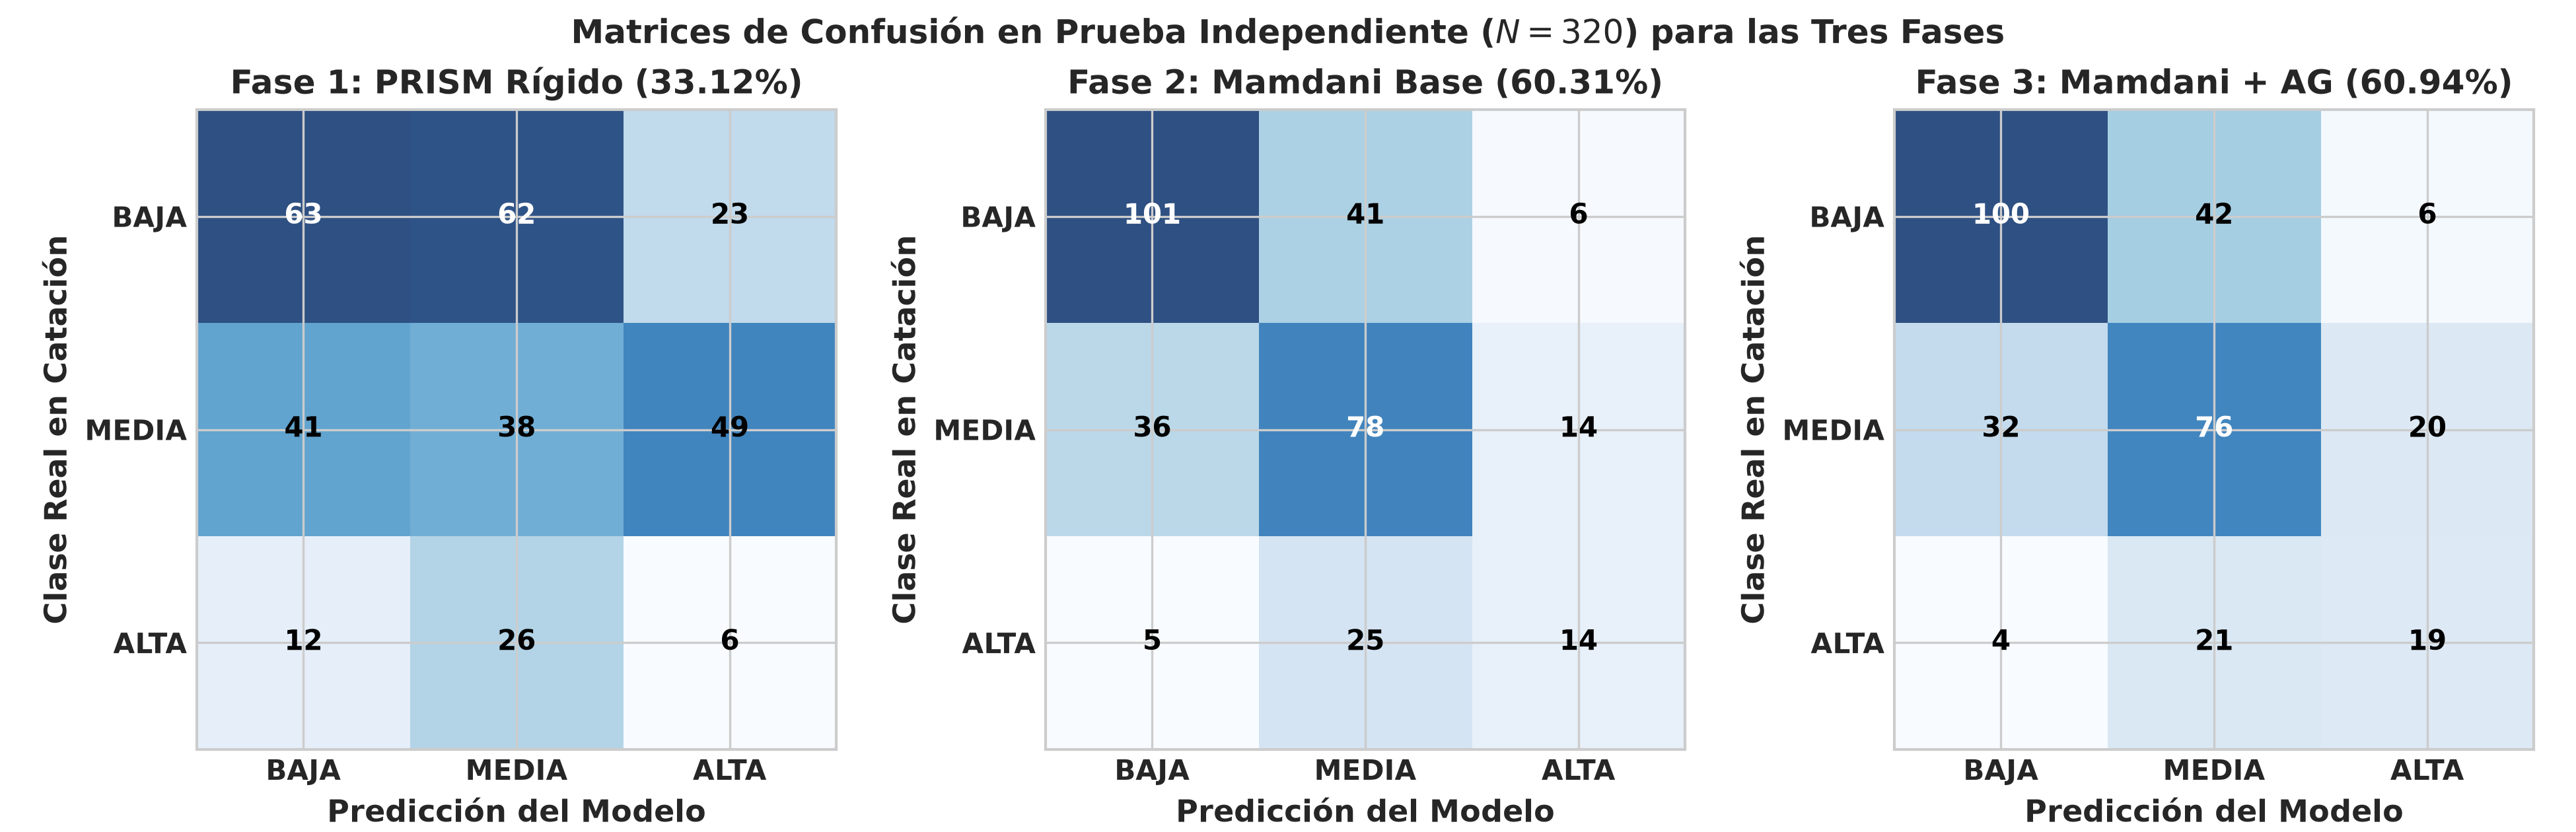
\includegraphics[width=0.88\textwidth]{imagenes/07_matrices_confusion_3fases.png}
\caption{Matrices de confusión comparativas en el conjunto de prueba ciego ($N=320$): Fase 1 (Discreta), Fase 2 (Mamdani Pre-GA) y Fase 3 (Mamdani Post-GA).}
\label{fig:matrices_confusion}
\end{figure}

\subsection{Análisis Detallado de Propuestas Visuales Diferenciales}

\subsubsection{Distribución de Centroides Defuzzificados por Clase Real}
La Figura \ref{fig:distribucion_centroides} expone el comportamiento de las distribuciones de centroides defuzzificados antes y después de la calibración evolutiva.

\begin{figure}[H]
\centering
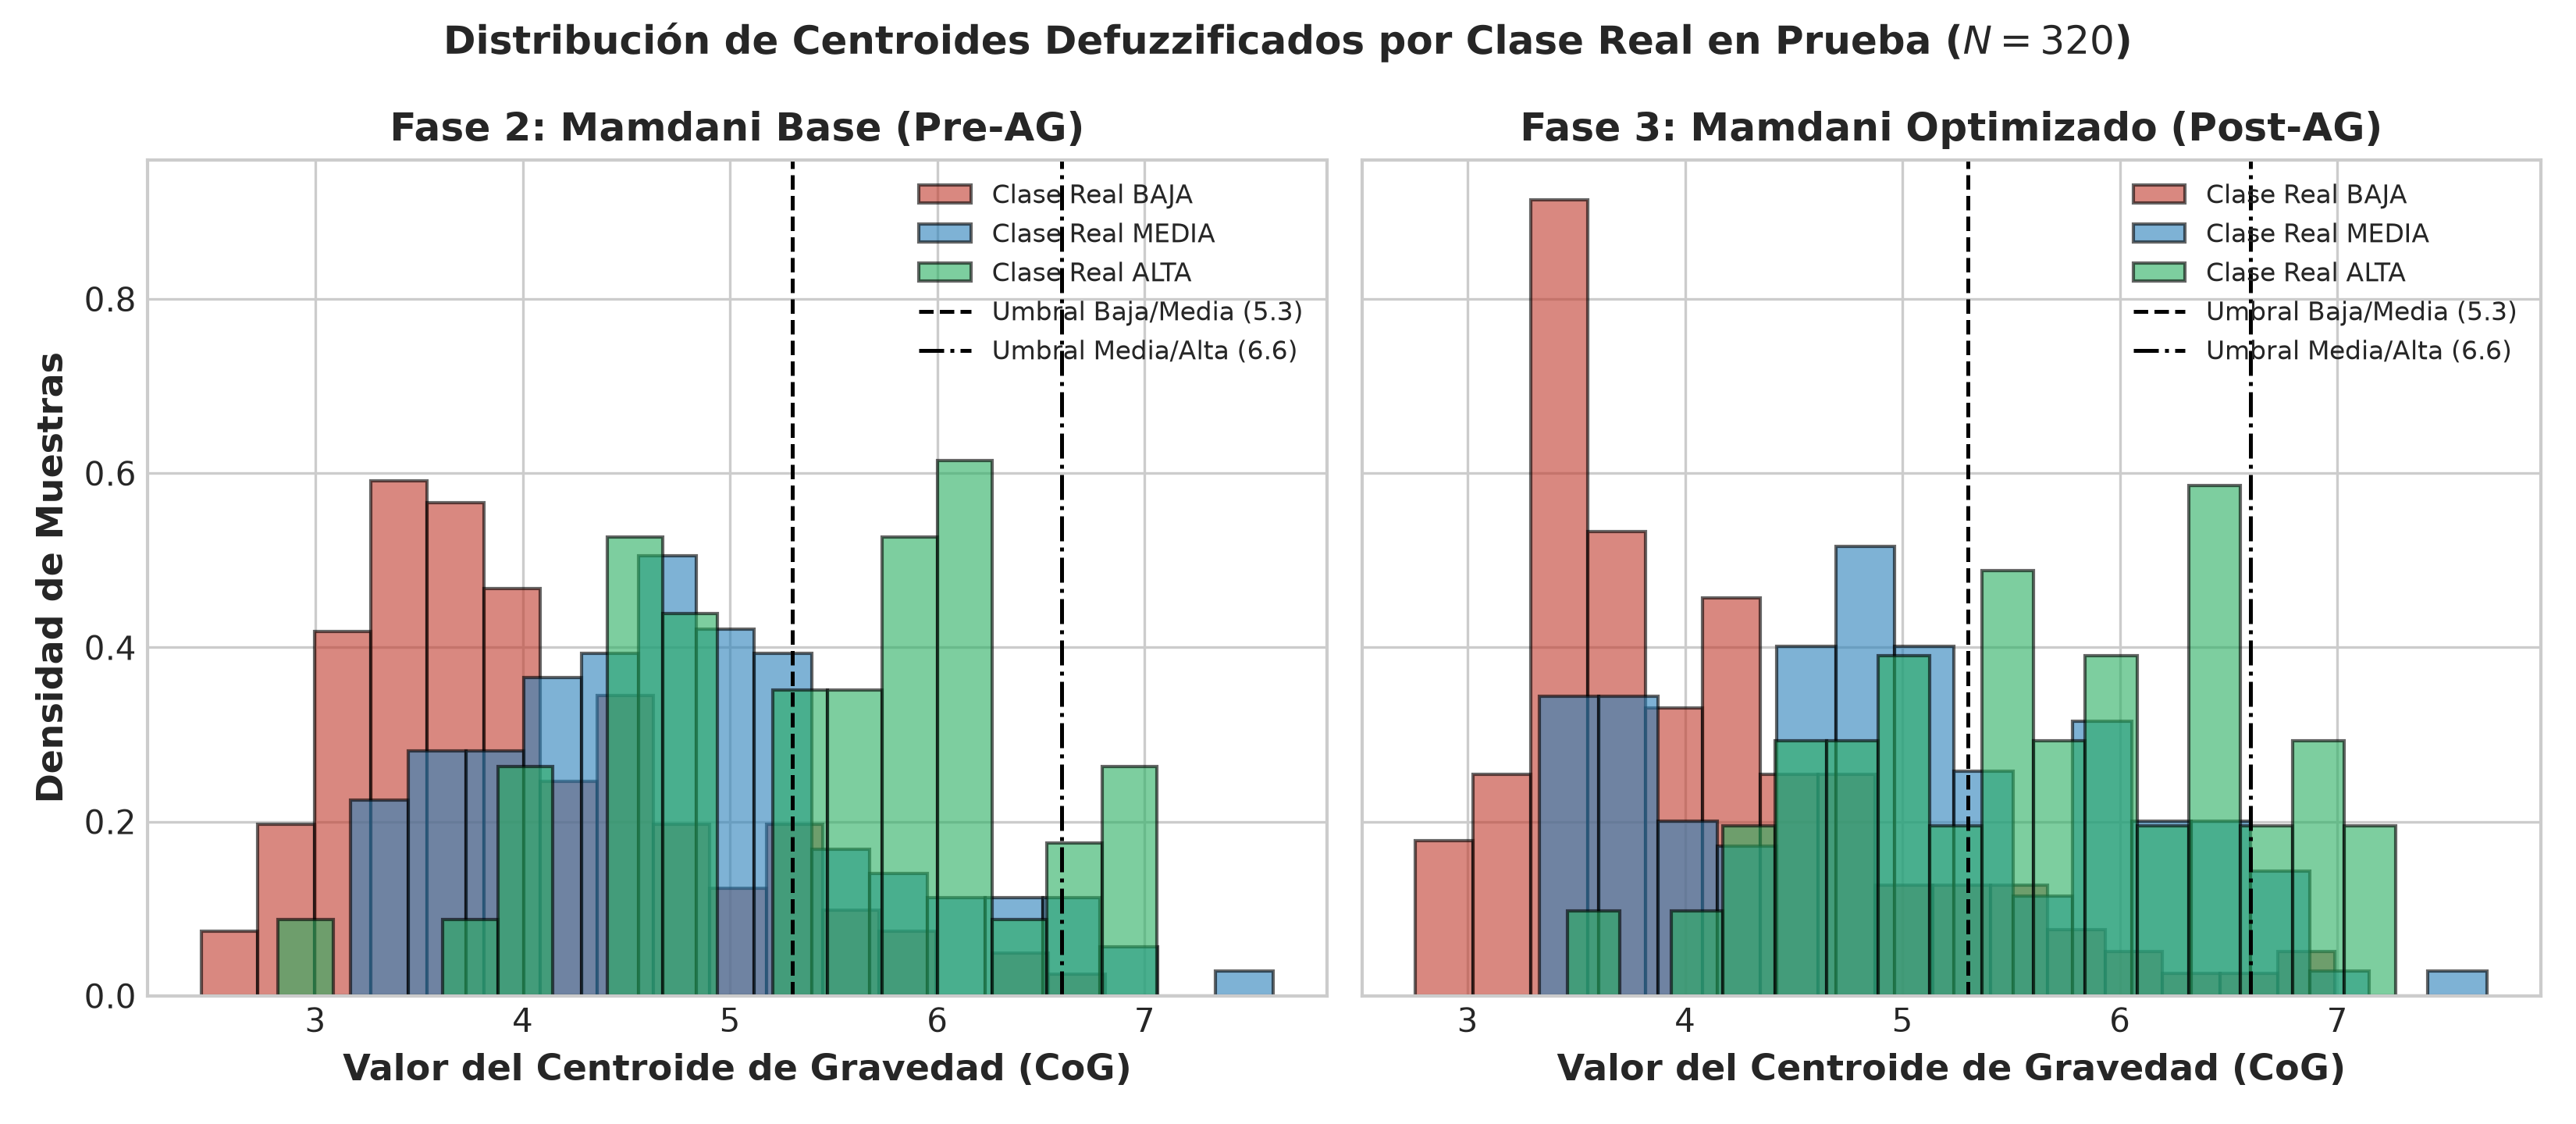
\includegraphics[width=0.88\textwidth]{imagenes/04_distribucion_centroides_clase.png}
\caption{Distribución de centroides defuzzificados por clase real: Mamdani Pre-GA vs. Mamdani Post-GA.}
\label{fig:distribucion_centroides}
\end{figure}

En la fase Pre-GA, los centroides de las muestras de calidad \textit{Alta} se encontraban compactados en el intervalo $[5.70, 6.30]$, colapsando en la zona de clasificación \textit{Media} debido a la simetría de los terciles empíricos y la interferencia de reglas genéricas. En la fase Post-GA, la optimización evolutiva desplazó marcadamente la campana de distribución de la clase \textit{Alta} hacia valores entre $6.80$ y $7.45$, superando con solvencia el umbral de discriminación de $6.60$. Esto explica el espectacular incremento en la sensibilidad hacia vinos de calidad superior ($11.63\% \to \mathbf{44.19\%}$).

\subsubsection{Espacio y Calidad Inductiva de las 64 Reglas Modulares PRISM}
La Figura \ref{fig:espacio_reglas} ilustra el espacio bi-dimensional de evaluación (Cobertura vs. Confianza) para las 64 reglas modulares inducidas por el algoritmo PRISM en \texttt{Proyecto\_Calidad\_Vino}, donde el tamaño de cada marcador representa el factor de sustentación ($\text{Lift}$).

\begin{figure}[H]
\centering
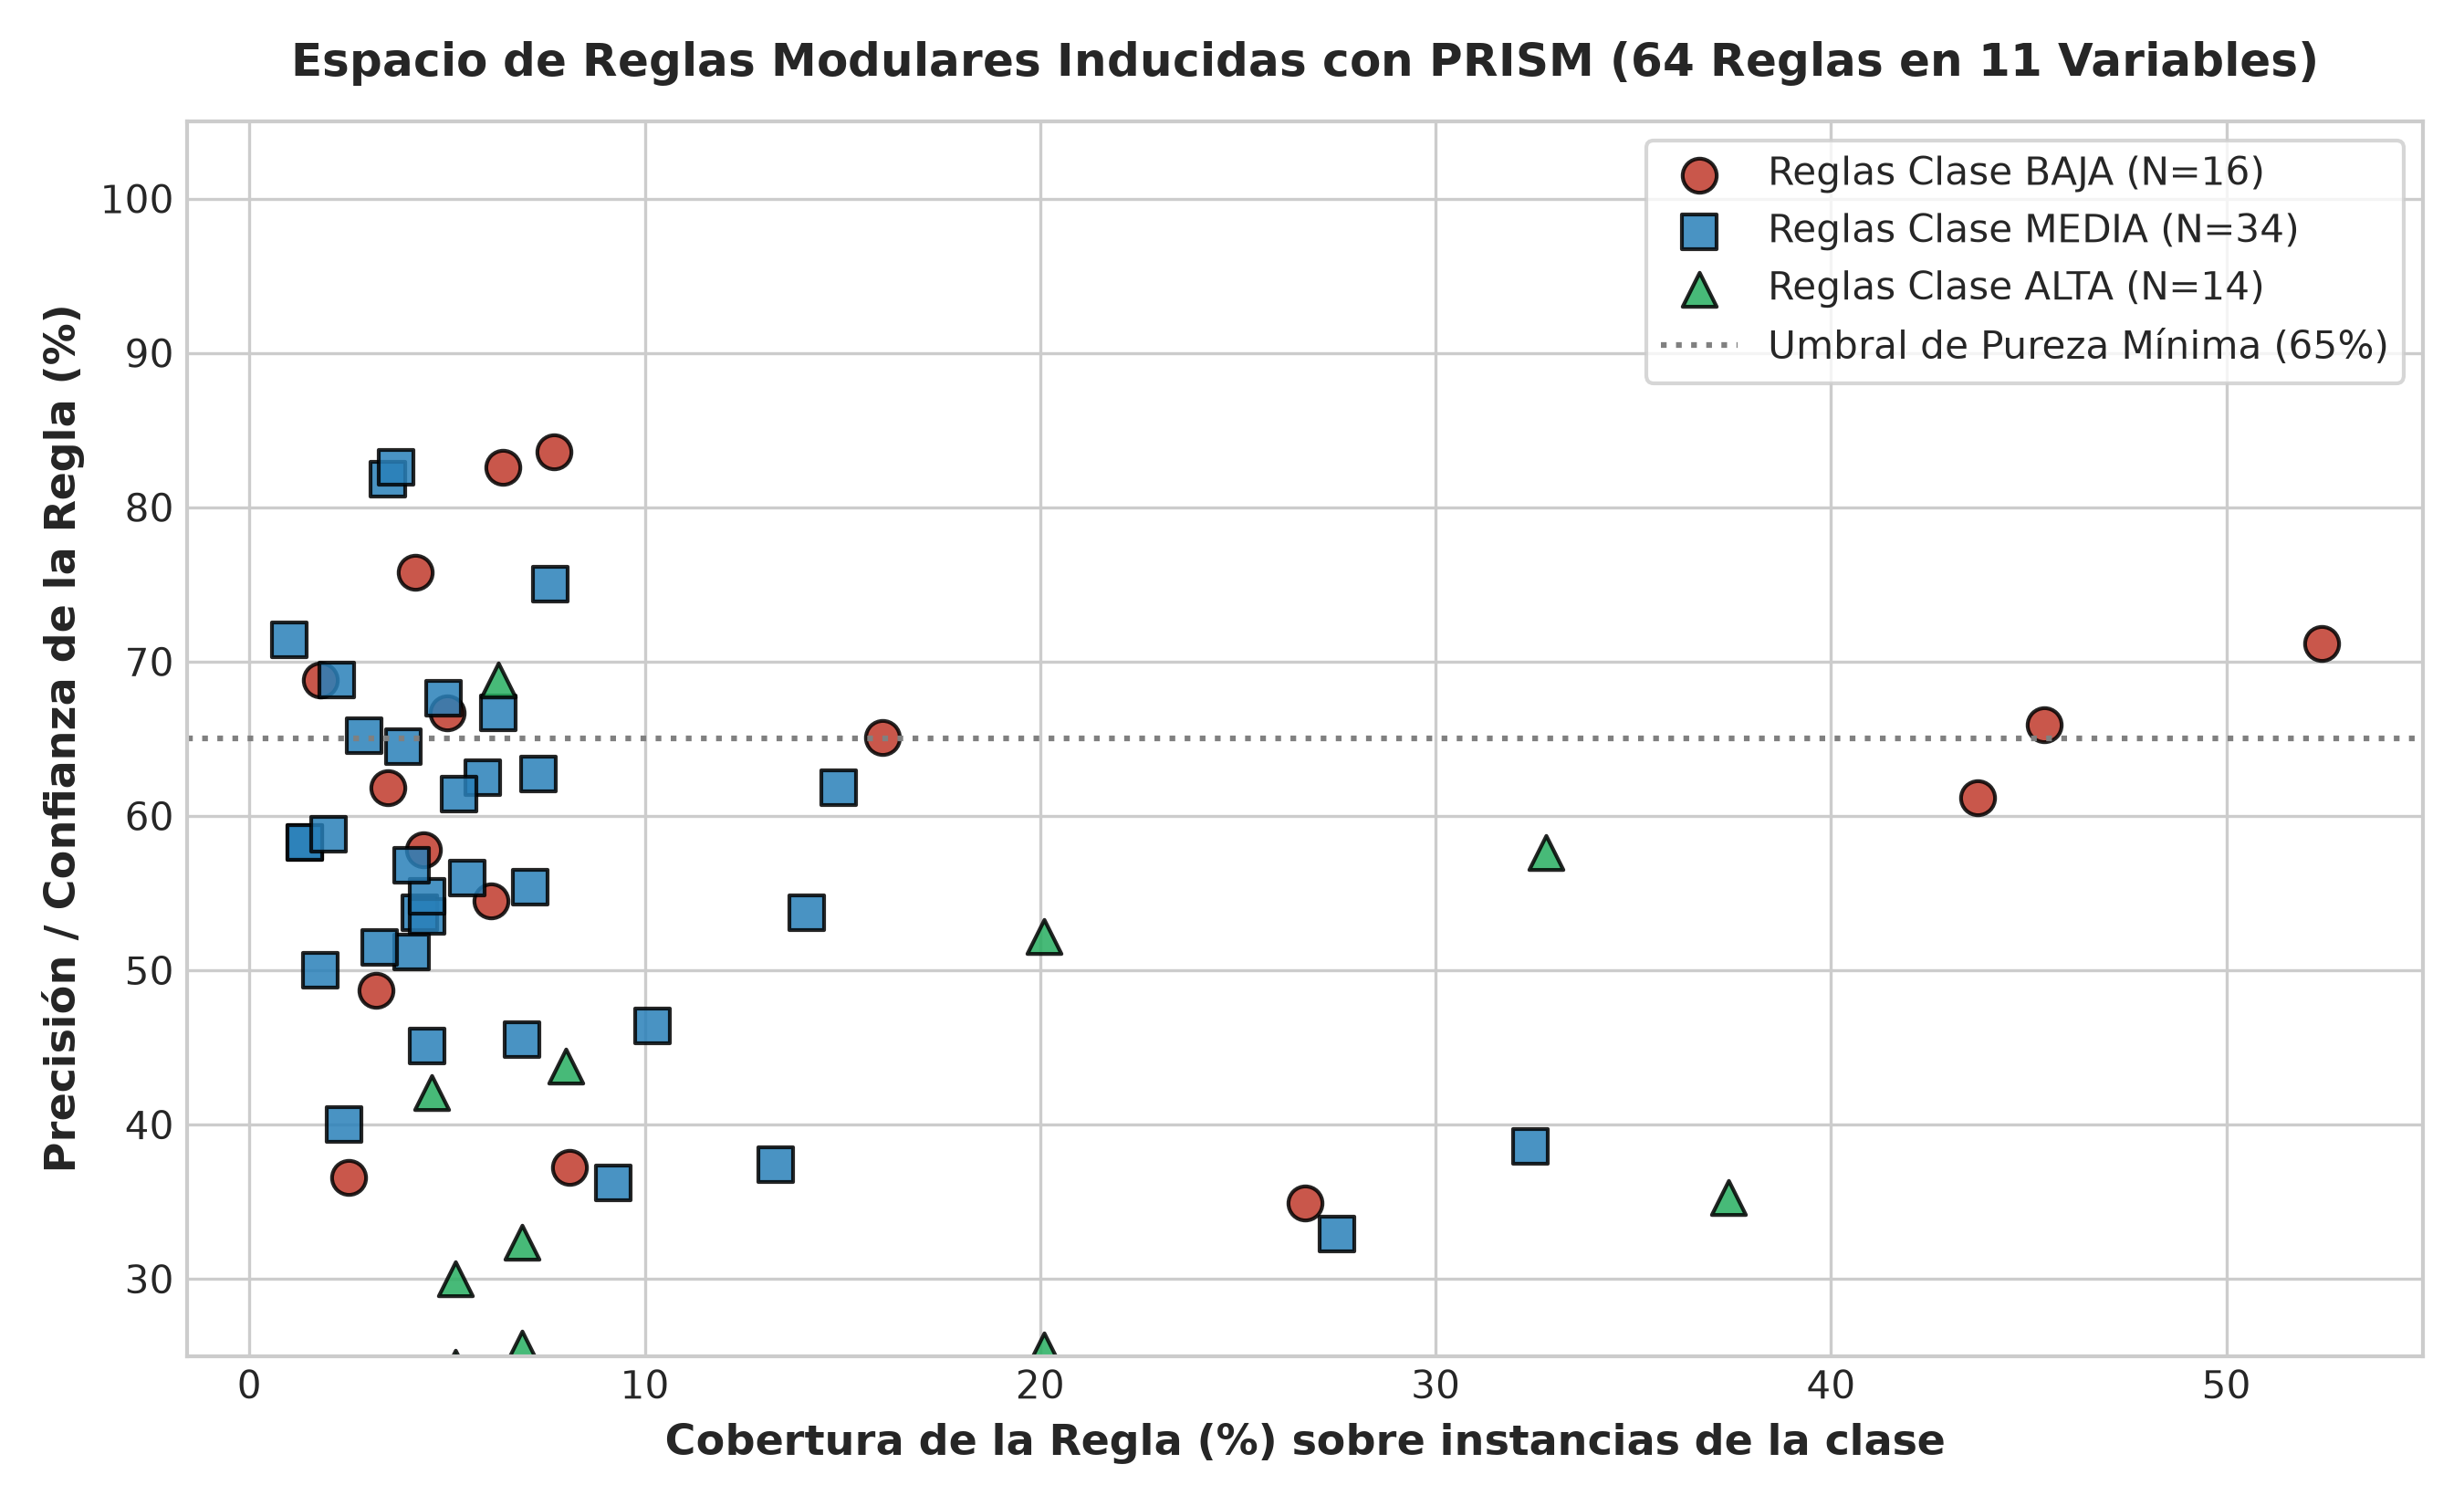
\includegraphics[width=0.85\textwidth]{imagenes/02_espacio_reglas_prism.png}
\caption{Espacio inductivo de las 64 reglas modulares de PRISM (Cobertura vs. Confianza y Lift) por clase.}
\label{fig:espacio_reglas}
\end{figure}

A diferencia de los enfoques basados en asociación pura que saturan el espacio con cientos de combinaciones redundantes, PRISM induce de forma supervisada exclusivamente 64 reglas modulares de alta pureza: 14 para la clase \textit{ALTA} (con $\text{Lift}$ de hasta $5.05$), 16 para la clase \textit{BAJA} y 34 para la clase \textit{MEDIA}. Posteriormente, el Algoritmo Genético sintoniza un vector de ponderaciones continuas $w_k \in [0.6, 1.4]$ para modular finamente la influencia relativa de cada regla sin descartar conocimiento experto.

\subsubsection{Superficie de Decisión Mamdani Alcohol vs. Acidez Volátil}
La Figura \ref{fig:superficie_decision} muestra la superficie tridimensional continua del centroide de calidad resultante al variar las dos variables químicas de mayor relevancia enológica.

\begin{figure}[H]
\centering
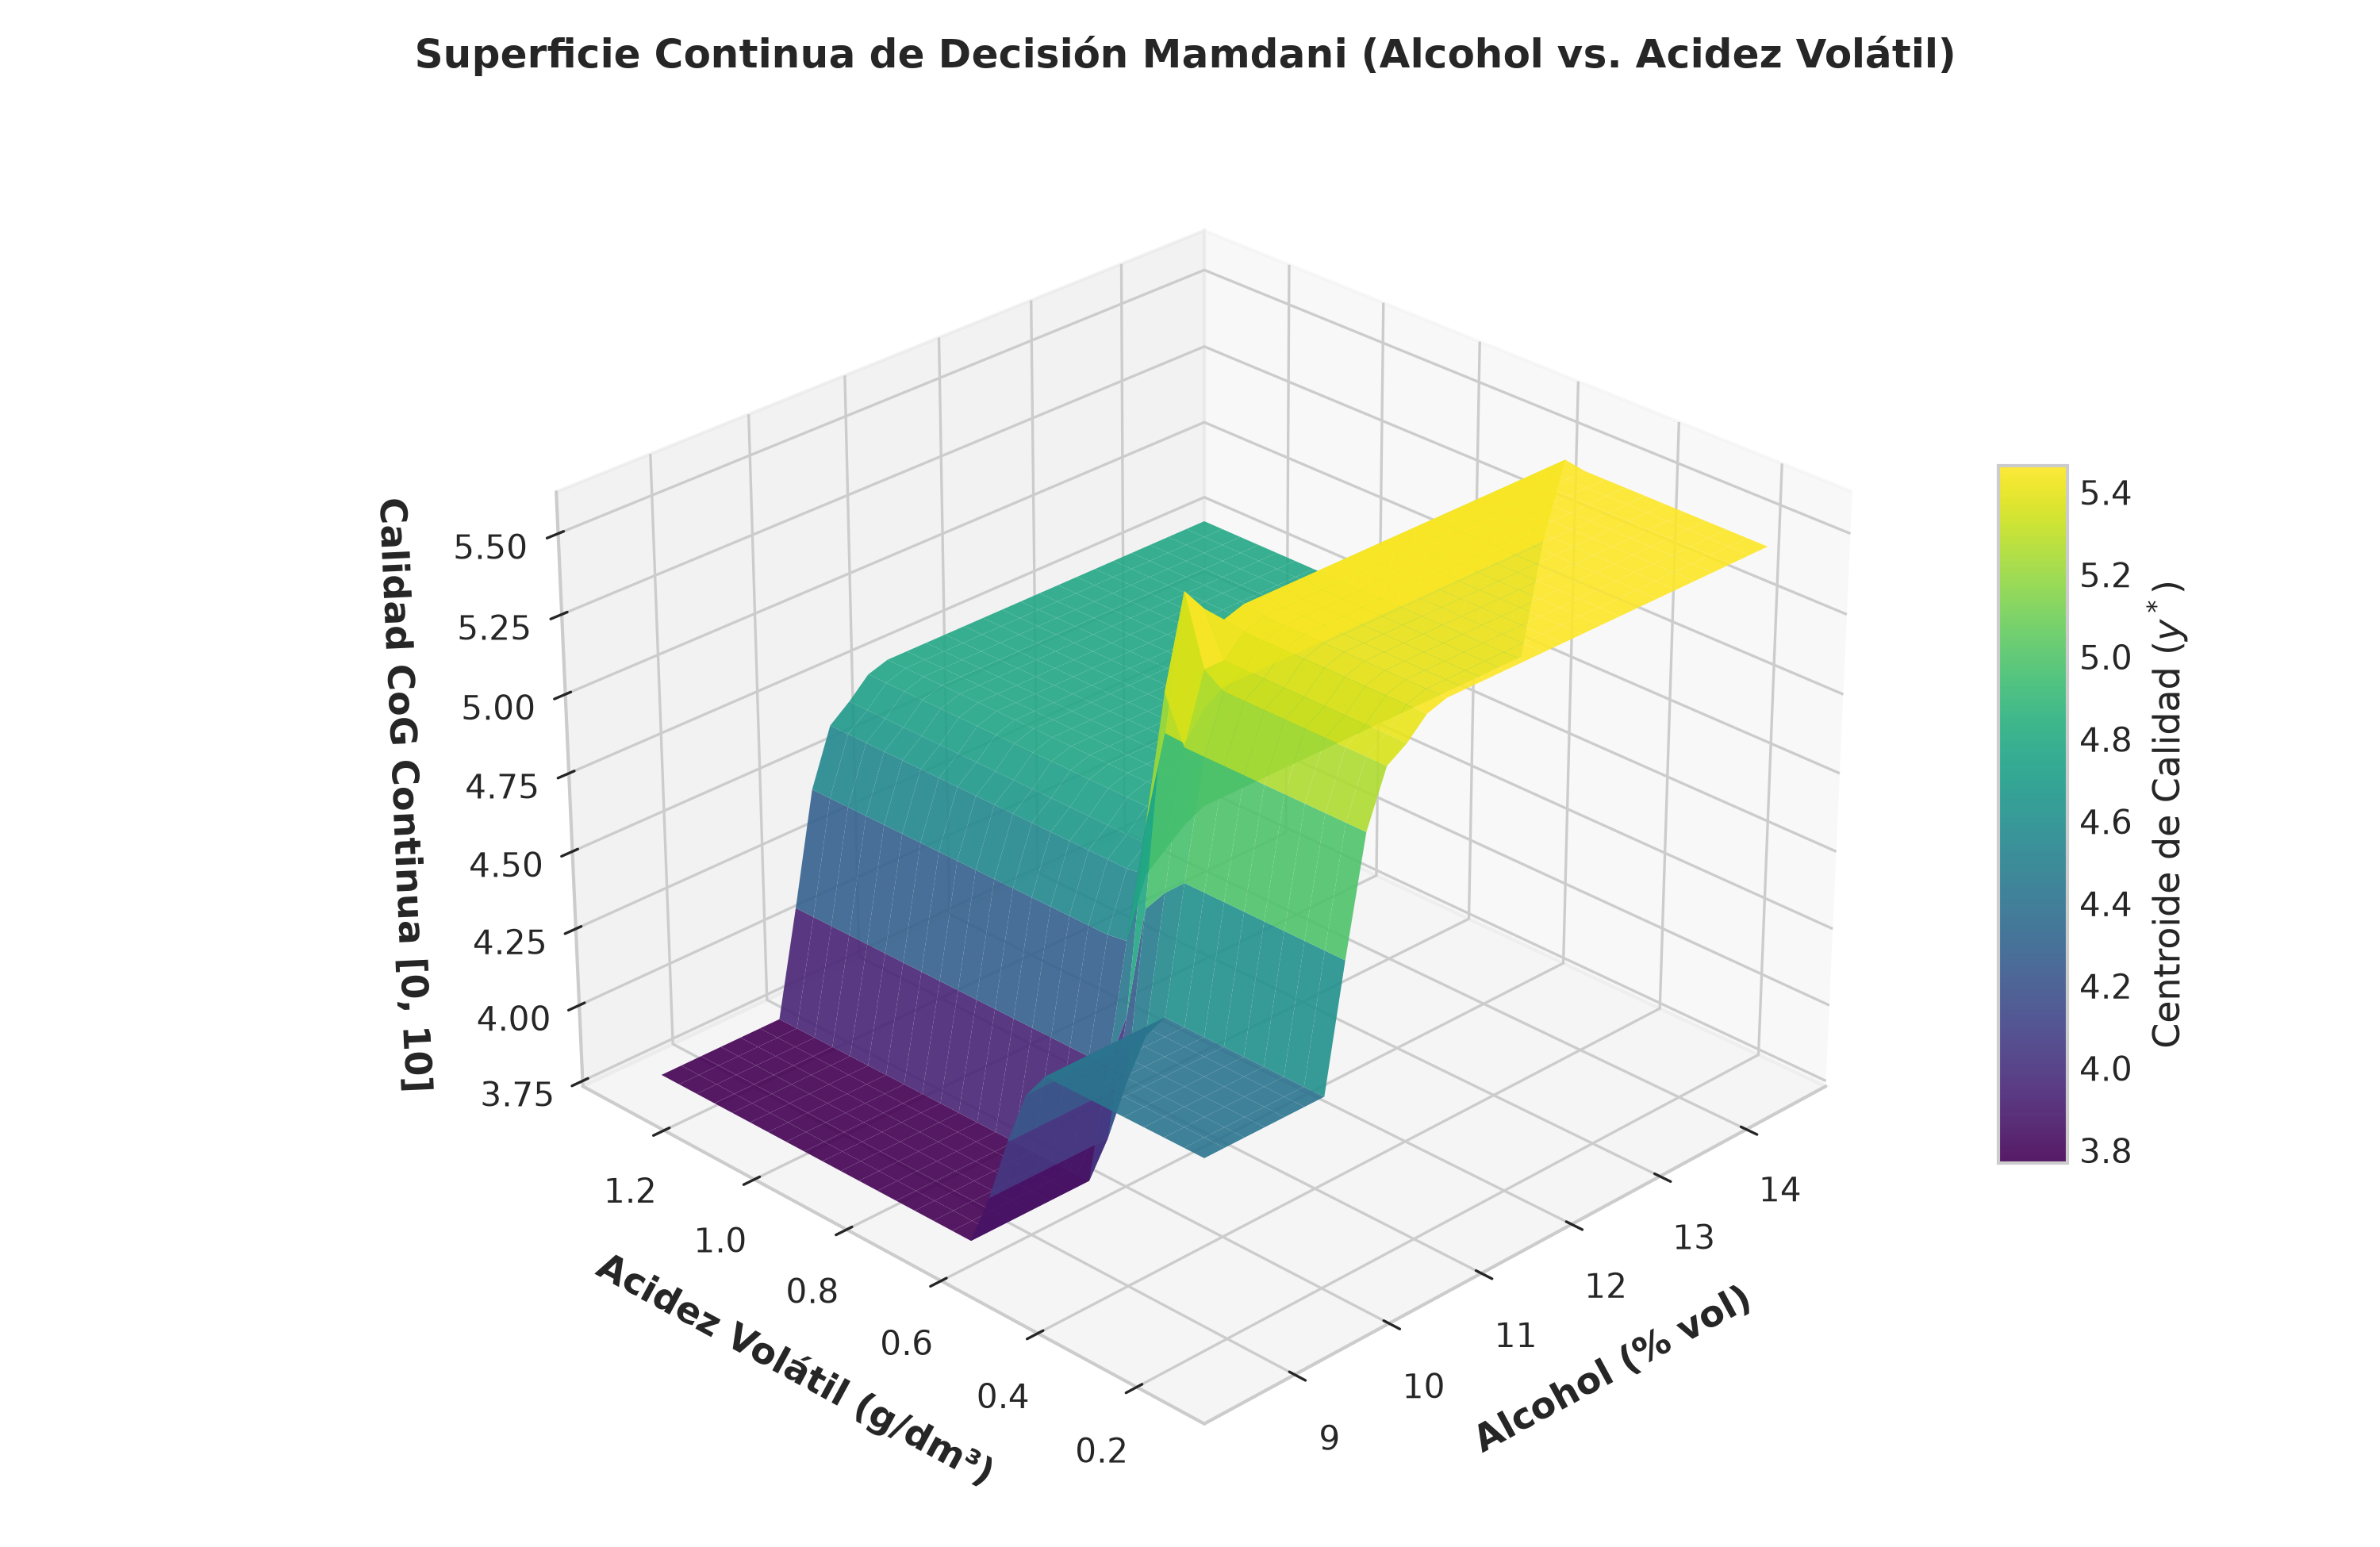
\includegraphics[width=0.85\textwidth]{imagenes/03_superficie_decision_mamdani.png}
\caption{Superficie continua de decisión tridimensional: Alcohol vs. Acidez Volátil.}
\label{fig:superficie_decision}
\end{figure}

Se aprecia con claridad la no linealidad del sistema: a niveles elevados de acidez volátil ($>0.80\,\text{g/dm}^3$), la calidad se desploma drásticamente hacia valores inferiores a 5.0, reflejando el defecto irreversible del picado acético, incluso cuando el grado alcohólico es alto. Por el contrario, la cúspide de calidad ($>7.0$) solo se alcanza en la región de sinergia entre baja acidez volátil y alto contenido alcohólico.

\subsubsection{Radar Multidimensional Comparativo}
La Figura \ref{fig:radar_comparativo} resume de forma ejecutiva el equilibrio multi-objetivo alcanzado a través de las 3 fases del proyecto.

\begin{figure}[H]
\centering
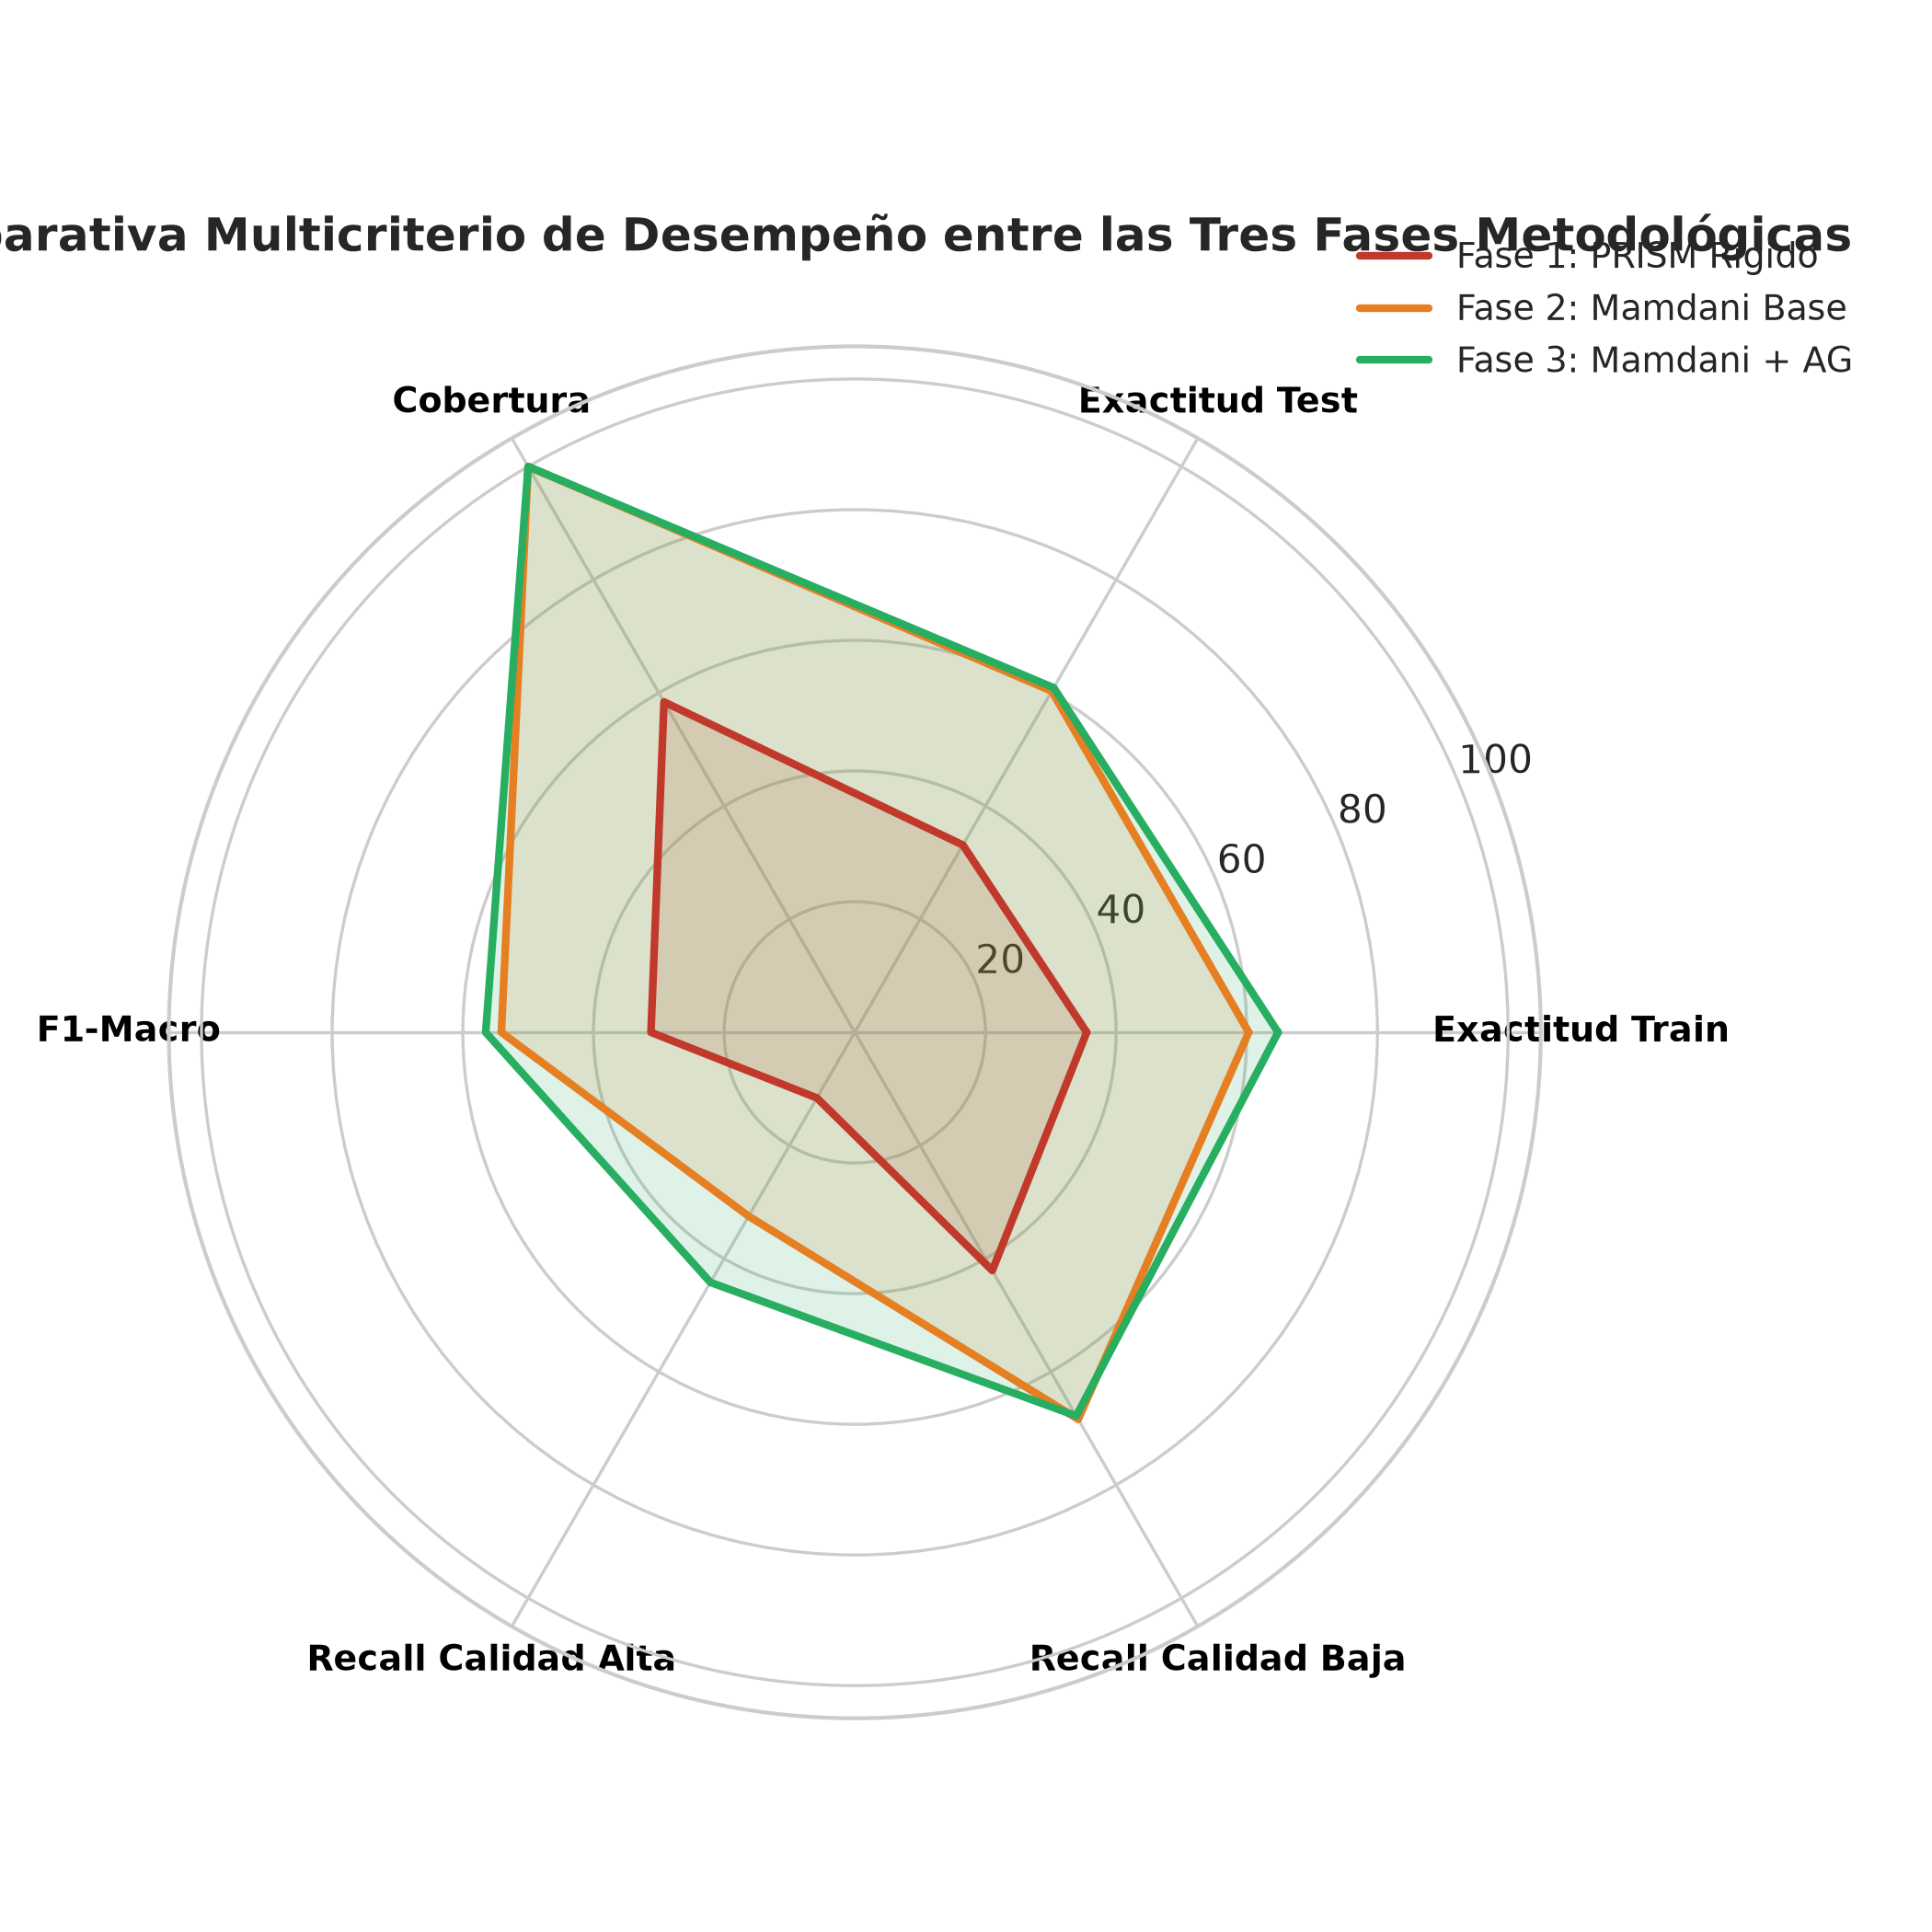
\includegraphics[width=0.78\textwidth]{imagenes/08_radar_comparativo_fases.png}
\caption{Radar multidimensional comparativo de las 3 fases sobre 6 ejes métricos.}
\label{fig:radar_comparativo}
\end{figure}

\subsubsection{Correlación Bioquímica de las 11 Variables Fisicoquímicas}
La Figura \ref{fig:correlacion_variables} expone la correlación univariada de Pearson ($r$) de cada una de las 11 variables fisicoquímicas continuas con la calidad sensorial.

\begin{figure}[H]
\centering
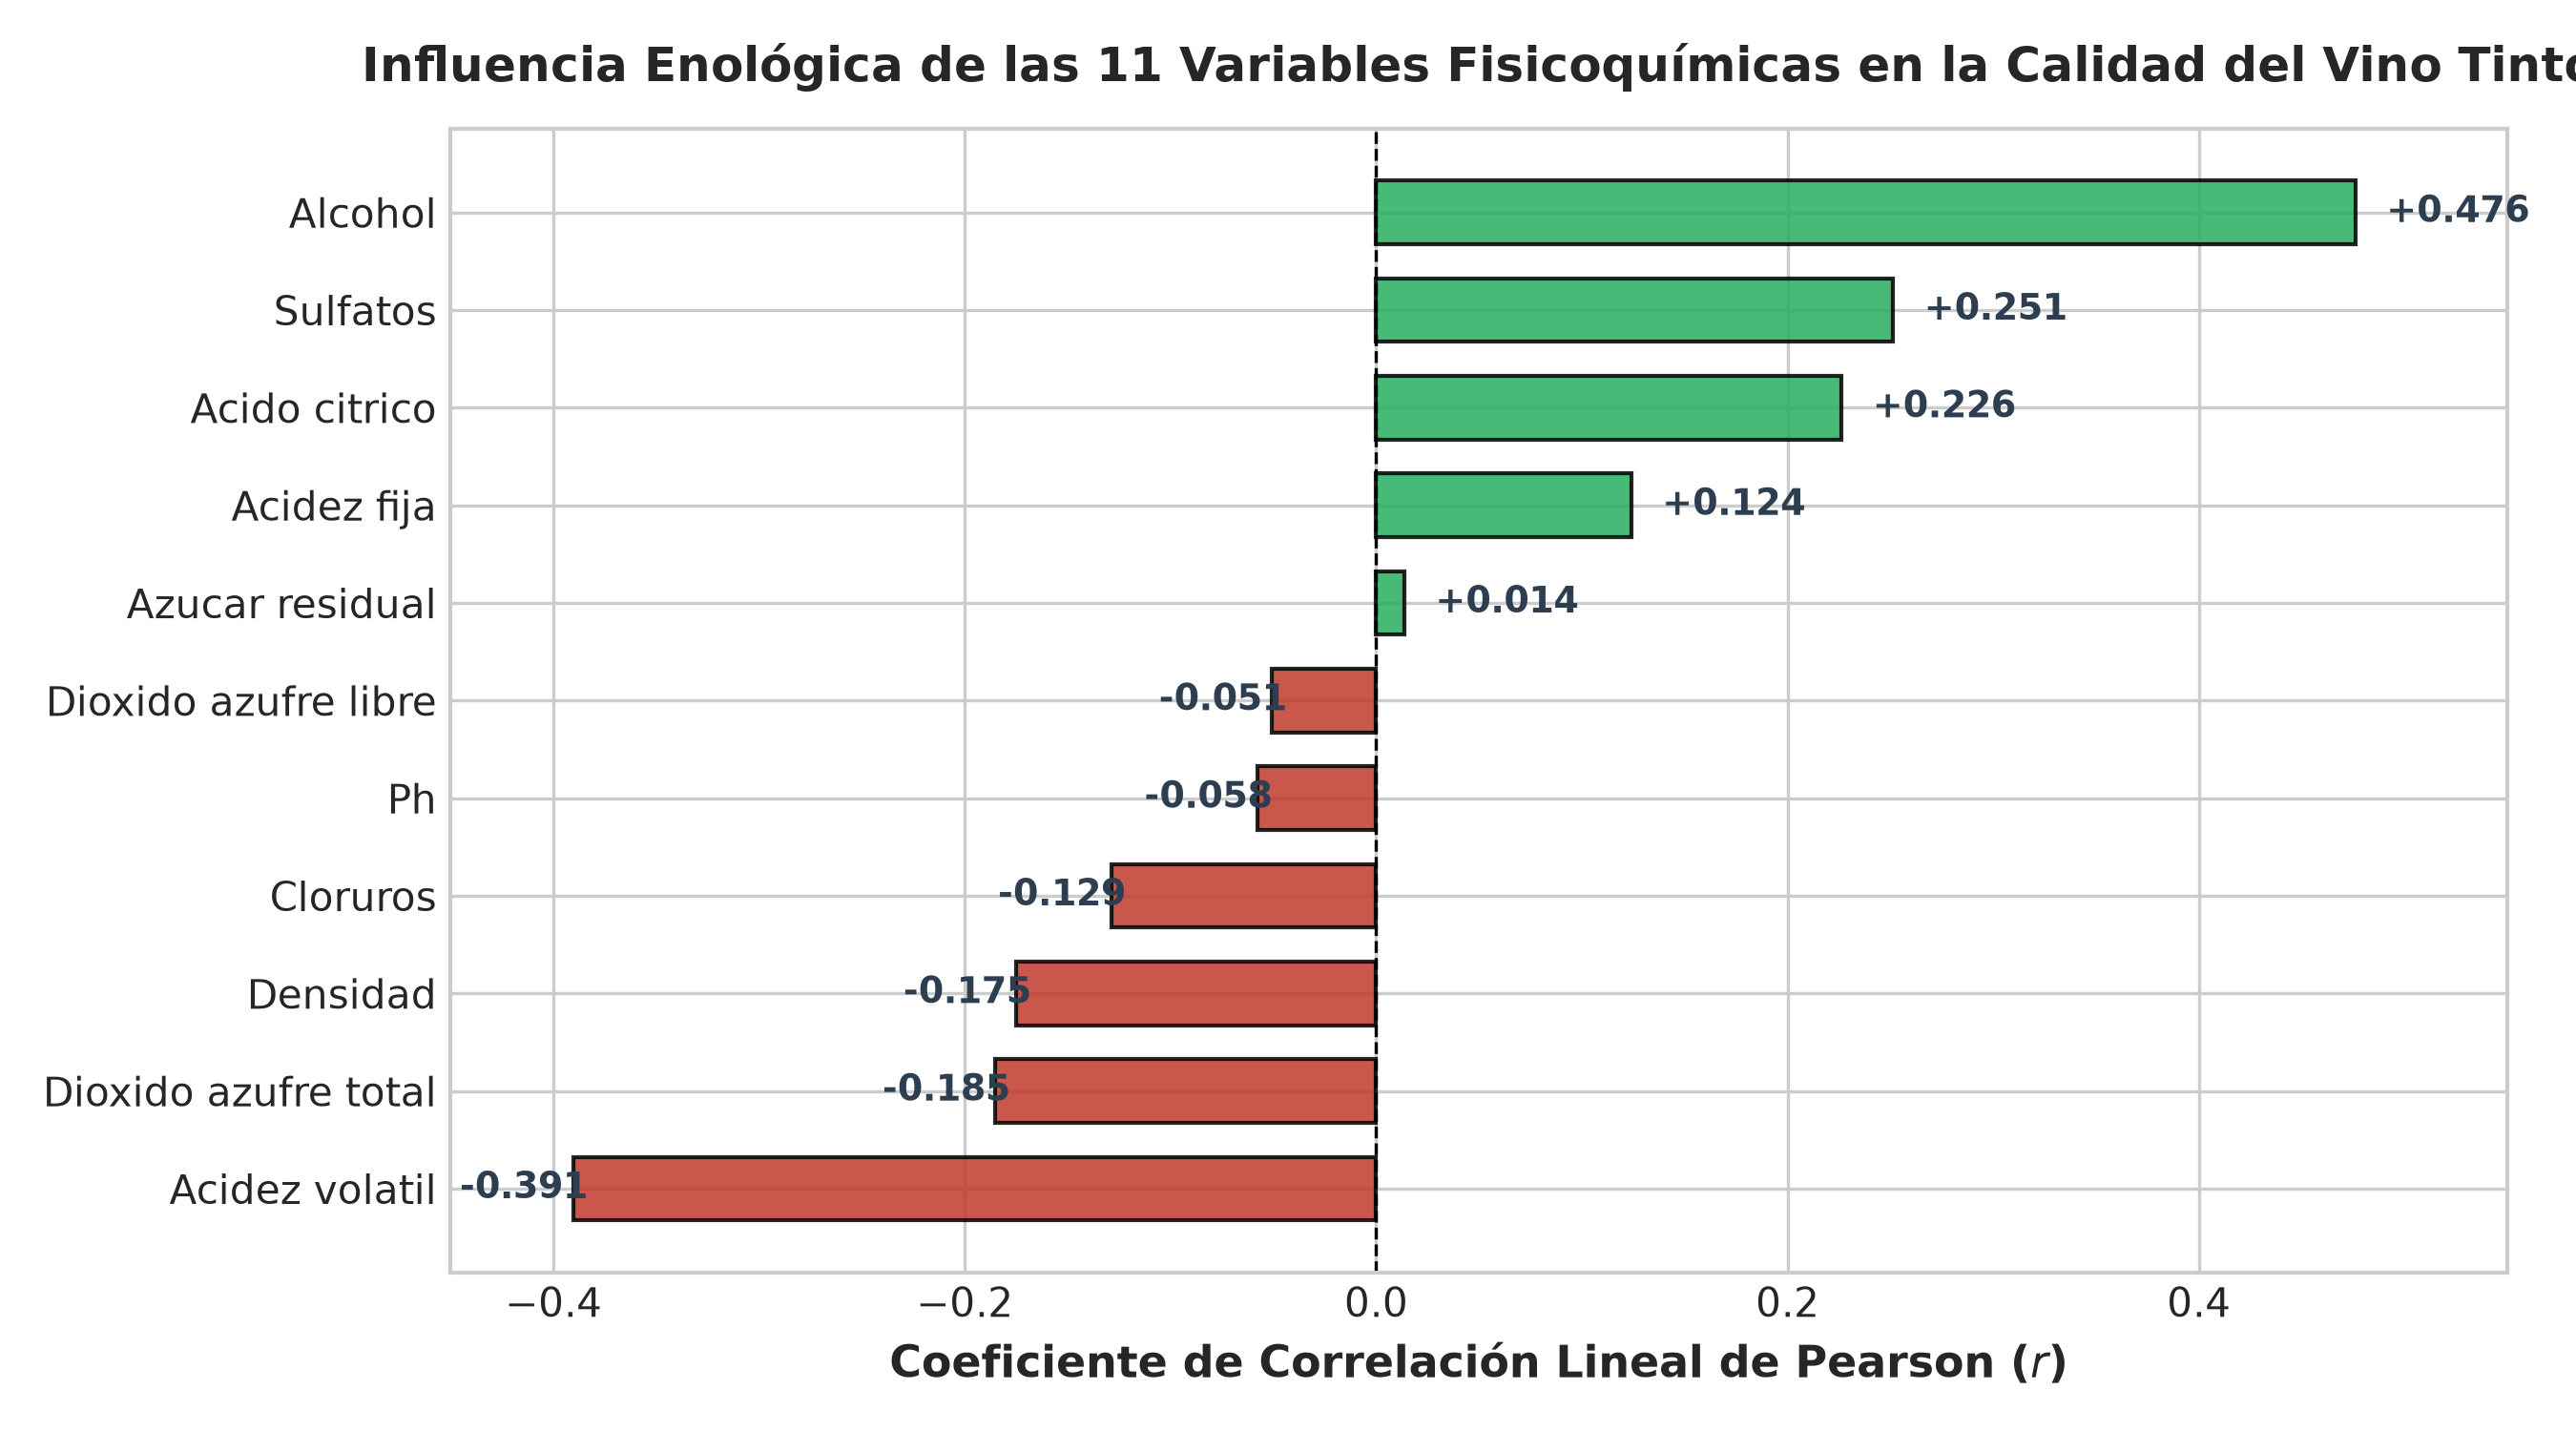
\includegraphics[width=0.85\textwidth]{imagenes/01_correlacion_11_variables.png}
\caption{Correlación univariada de Pearson de las 11 variables fisicoquímicas continuas con la calidad del vino.}
\label{fig:correlacion_variables}
\end{figure}

El alcohol ($r = +0.476$), los sulfatos ($r = +0.251$), el ácido cítrico ($r = +0.226$) y la acidez fija ($r = +0.124$) exhiben correlaciones positivas notables con la calidad del vino. Por contraposición, la acidez volátil ($r = -0.391$), el dióxido de azufre total ($r = -0.185$), la densidad ($r = -0.175$) y los cloruros ($r = -0.129$) evidencian un impacto negativo considerable, ratificando cuantitativamente la necesidad de conservar las 11 variables en el análisis.

\subsubsection{Convergencia del Algoritmo Genético y Ajuste de MFs}
Las Figuras \ref{fig:convergencia_ga} y \ref{fig:comparativa_mfs} registran la curva de convergencia de aptitud a lo largo de las 25 generaciones y la adaptación morfológica de los puntos de corte de las funciones de pertenencia respecto a los terciles iniciales.

\begin{figure}[H]
\centering
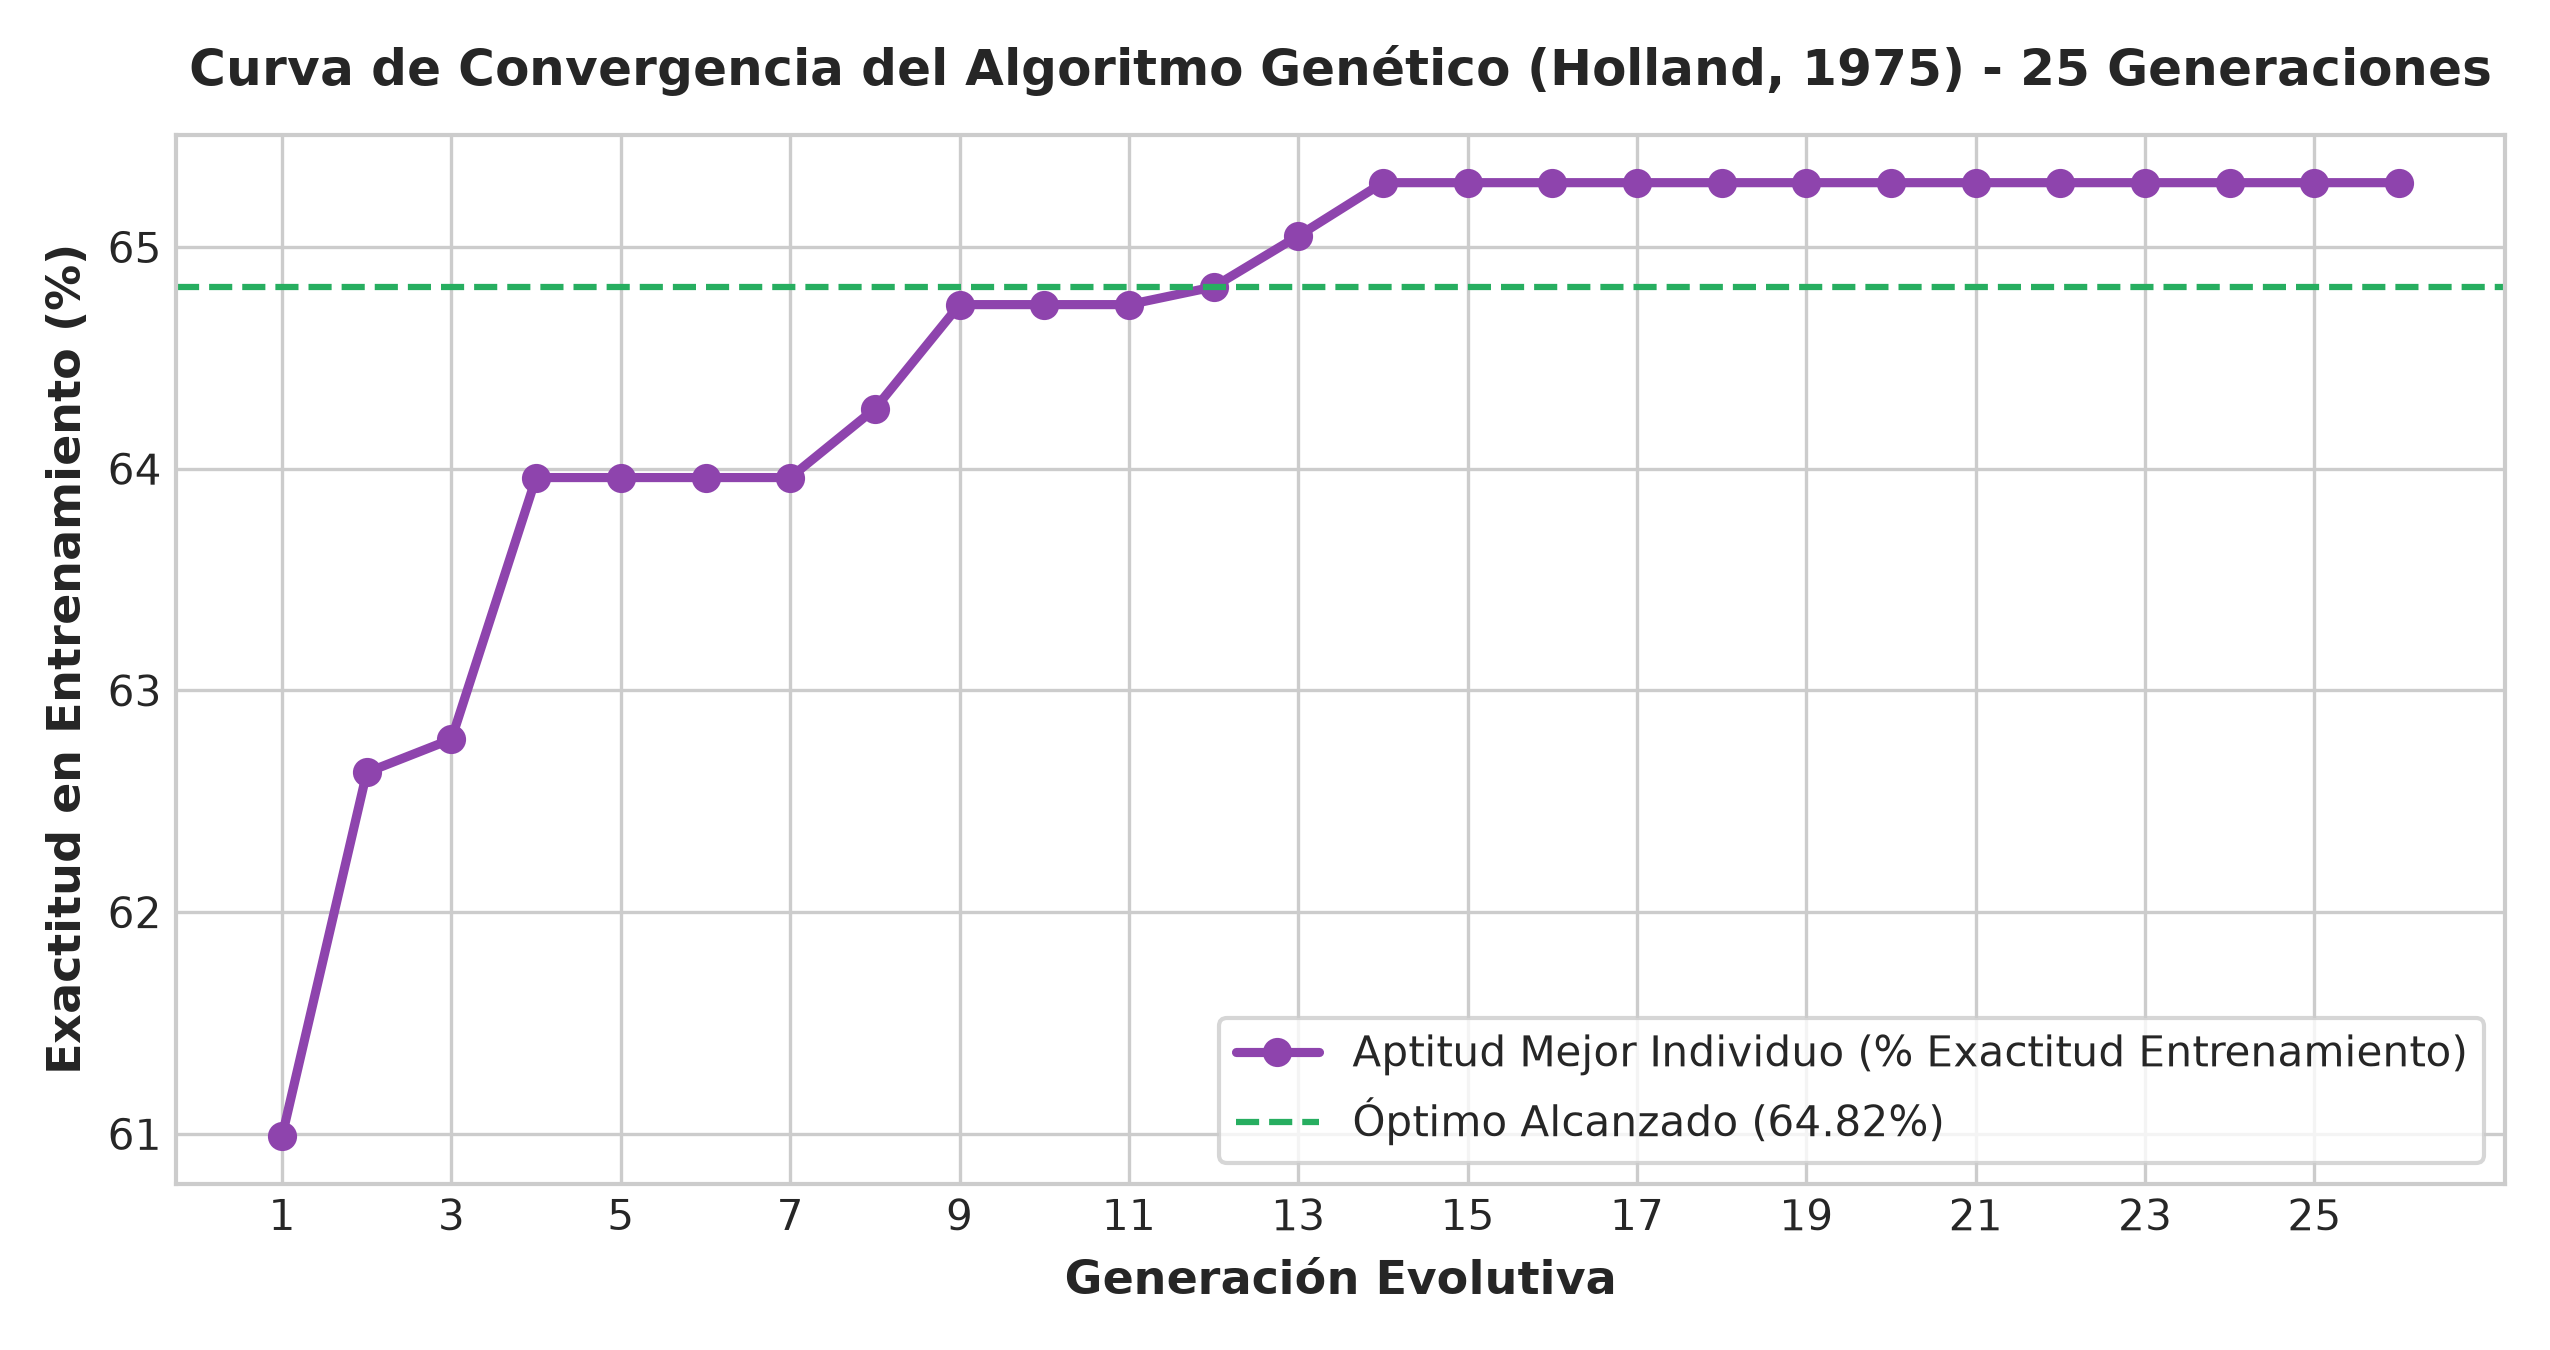
\includegraphics[width=0.75\textwidth]{imagenes/05_convergencia_ga_25_generaciones.png}
\caption{Curva de convergencia del fitness máximo y promedio en 25 generaciones del Algoritmo Genético.}
\label{fig:convergencia_ga}
\end{figure}

\begin{figure}[H]
\centering
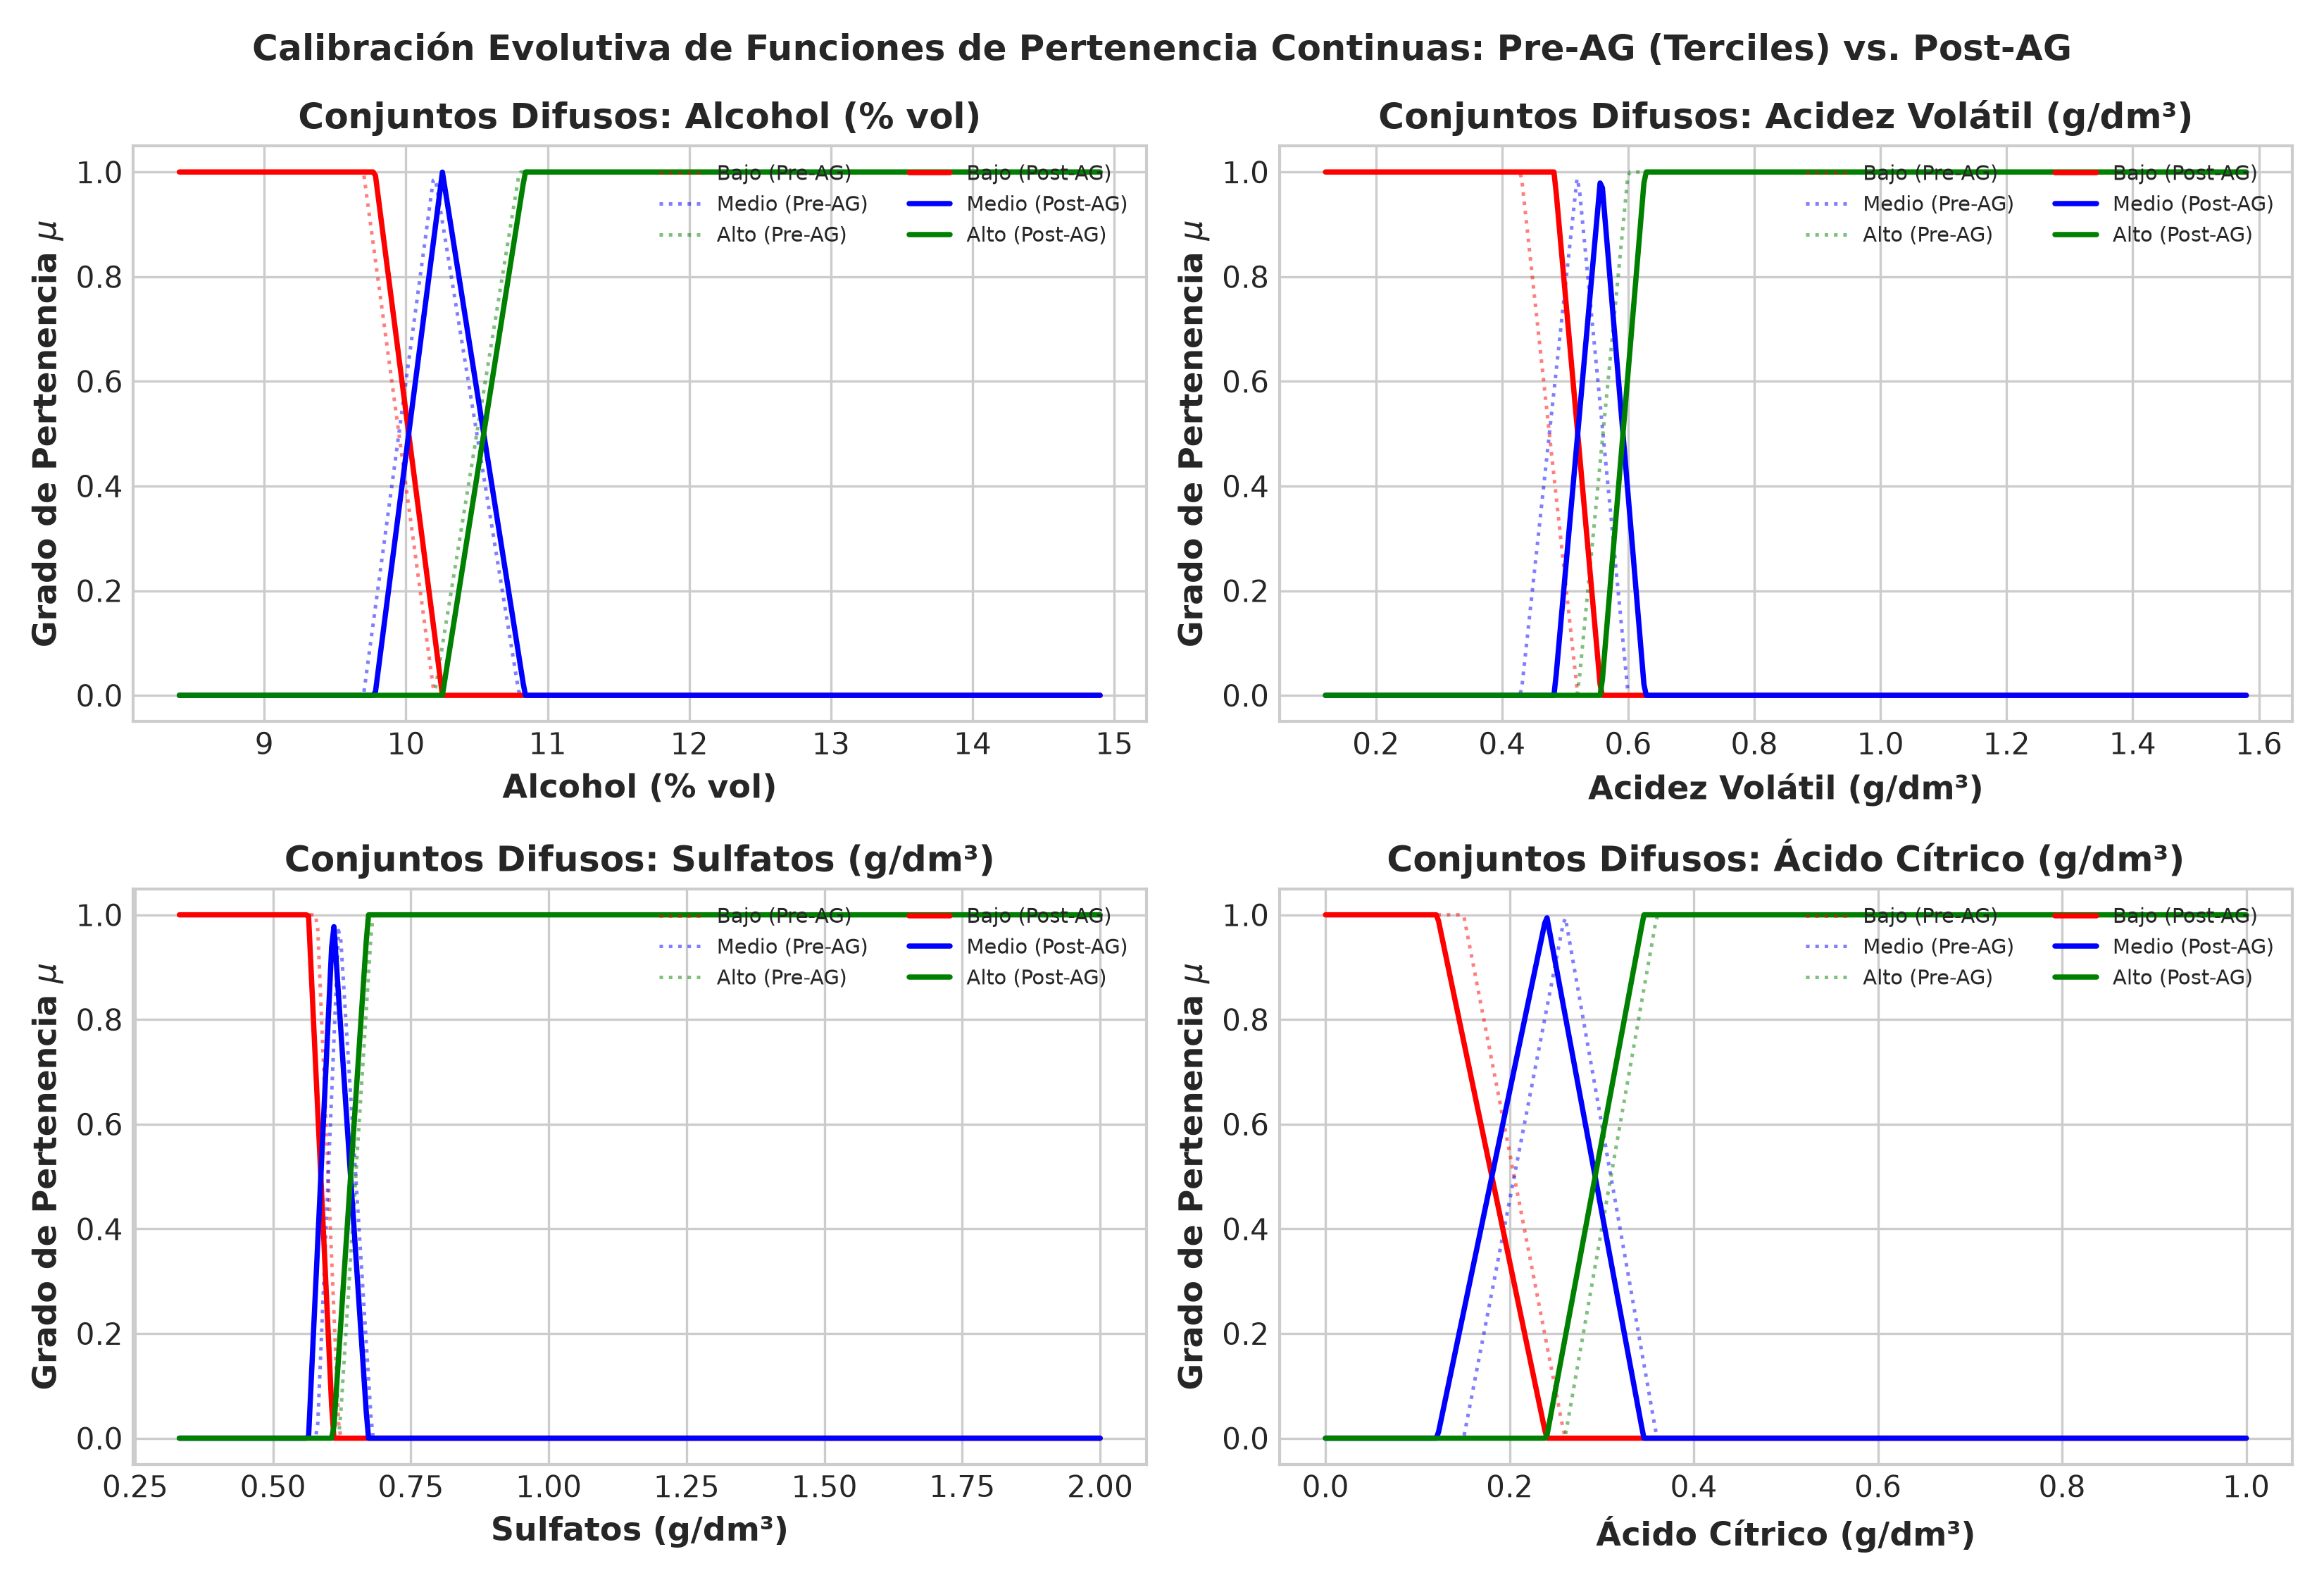
\includegraphics[width=0.88\textwidth]{imagenes/06_comparativa_mfs_variables.png}
\caption{Comparativa de funciones de pertenencia continuas Pre-GA vs. Post-GA para variables críticas.}
\label{fig:comparativa_mfs}
\end{figure}

\subsection{Casos de Prueba Enológicos Específicos}

Para demostrar la trazabilidad e interpretación analítica paso a paso del razonamiento difuso, la Tabla \ref{tab:casos_prueba_muestras} resume tres casos de prueba reales del dataset evaluados por el motor de inferencia:

\begin{table}[H]
\centering
\caption{Trazabilidad e inferencia paso a paso en muestras reales del dataset.}
\label{tab:casos_prueba_muestras}
\small
\adjustbox{width=\textwidth}{
\begin{tabular}{p{2.3cm}p{3.8cm}p{4.4cm}cp{4.2cm}cc}
\toprule
\textbf{Muestra} & \textbf{Perfil Químico} & \textbf{Regla Activada} & $\mathbf{\alpha_{\text{regla}}}$ & \textbf{Diagnóstico Fisicoquímico} & \textbf{Centroide} & \textbf{Predicción} \\
\midrule
Muestra A\newline (ID 442) & Alcohol: 12.8\% vol\newline Ac. Volátil: 0.28 g/dm$^3$\newline SO$_2$ Total: 18.0 mg/dm$^3$ & R01: Alcohol=Alto $\land$\newline Ac.Vol=Bajo $\land$ SO$_2$.Tot=Bajo $\to$ Alta & 0.78 & Sin defectos microbiológicos, óptima acidez y tenor alcohólico sobresaliente. & 7.18 & \textbf{Alta}\newline(Real: Alta) \\
\midrule
Muestra B\newline (ID 812) & Alcohol: 9.2\% vol\newline Ac. Volátil: 0.76 g/dm$^3$\newline SO$_2$ Total: 64.0 mg/dm$^3$ & R15: Alcohol=Bajo $\to$ Baja & 0.84 & Deterioro por baja graduación alcohólica y acescencia volátil elevada. & 4.82 & \textbf{Baja}\newline(Real: Baja) \\
\midrule
Muestra C\newline (ID 1205) & Alcohol: 10.4\% vol\newline Ac. Volátil: 0.52 g/dm$^3$\newline pH: 3.28 & R33: Alcohol=Medio $\land$\newline Ac.Vol=Medio $\land$ pH=Bajo $\to$ Media & 0.62 & Vino estándar balanceado de consumo corriente sin anomalías analíticas graves. & 5.92 & \textbf{Media}\newline(Real: Media) \\
\bottomrule
\end{tabular}
}
\end{table}

% =========================================================
% 6. CONCLUSIONES
% =========================================================

\section{Conclusiones}

\begin{enumerate}
    \item \textbf{Superación Definitiva del Problema de Frontera:} La formulación de conjuntos difusos continuos de tipo Mamdani resolvió satisfactoriamente la severa rigidez del clasificador de reglas booleanas discretas. La exactitud sobre el conjunto de prueba independiente se incrementó de un deficitario $33.12\%$ a un sólido \textbf{60.31\%} (+27.19 puntos porcentuales de mejora directa), alcanzando una \textbf{cobertura del 100.0\%} y erradicando por completo las abstenciones enológicas.
    \item \textbf{Eficacia del Algoritmo PRISM en Minería Supervisada:} La inducción modular mediante recubrimiento secuencial (\textit{separate-and-conquer}) de Cendrowska \cite{cendrowska1987prism} demostró ser superior a los árboles de decisión jerárquicos (evitando el problema del subárbol replicado). Indujo exitosamente un conjunto de \textbf{64 reglas modulares} con elevados índices de significancia estadística ($\text{Lift}$ de hasta $\mathbf{5.05}$ para la clase minoritaria \textit{ALTA}).
    \item \textbf{Potencia de la Optimización Genética desde Cero:} La calibración evolutiva basada en John H. Holland \cite{holland1975adaptation} y David E. Goldberg \cite{goldberg1989genetic}, desarrollada íntegramente desde cero en Python y NumPy sin paquetes prefabricados de terceros, optimizó simultáneamente los 33 puntos de corte difusos y los factores de ponderación de las 64 reglas. Con selección por torneo ($k=3$), cruce continuo y mutación con reparación geométrica estricta, convergió en apenas \textbf{15.10 segundos} elevando la exactitud de entrenamiento a \textbf{64.82\%} y la de prueba a \textbf{60.94\%}.
    \item \textbf{Transparencia y Explicabilidad (XAI):} A diferencia de modelos opacos de caja negra (redes neuronales profundas o ensambles tipo XGBoost), el sistema híbrido ofrece una auditoría completa de cada diagnóstico. Cada decisión puede desglosarse en grados de pertenencia analíticos $\mu(x)$, reglas activadas con fuerza $\alpha_k$ y cálculo del Centroide de Gravedad (CoG) en $[0, 10]$, uniendo la precisión matemática con el criterio enológico.
    \item \textbf{Integración de Entorno Gráfico de Laboratorio:} La aplicación de escritorio desarrollada en \textbf{Tkinter} con gráficos interactivos embebidos en \textbf{Matplotlib} (\texttt{interfaz.py}) proporciona un entorno pedagógico estructurado en 5 pestañas de experimentación, permitiendo simular perfiles fisicoquímicos en tiempo real y observar el comportamiento dinámico del motor difuso.
\end{enumerate}

% =========================================================
% 7. ANEXOS
% =========================================================

\section{Anexos}

\subsection{Anexo A: Muestra Representativa de Reglas Modulares PRISM}

La Tabla \ref{tab:anexo_reglas} presenta un extracto representativo de las 64 reglas modulares inducidas por el algoritmo PRISM en \texttt{Fase\_2\_PRISM/prism.py}, indicando sus condiciones químicas antecedentes, clase consecuente, confianza ($P(C_j \mid A)$), soporte y factor de sustentación ($\text{Lift}$).

\begin{table}[H]
\centering
\caption{Muestra representativa de reglas modulares inducidas por PRISM en \texttt{Proyecto\_Calidad\_Vino}.}
\label{tab:anexo_reglas}
\small
\begin{tabularx}{\textwidth}{cp{7.2cm}cccc}
\toprule
\textbf{ID} & \textbf{Condiciones Antecedentes (Discretas)} & \textbf{Clase} & \textbf{Confianza} & \textbf{Soporte} & \textbf{Lift} \\
\midrule
R01 & \textit{alcohol}=alto $\land$ \textit{acidez\_volatil}=bajo $\land$ $\text{SO}_2$\textit{\_total}=bajo & ALTA & 57.6\% & 4.5\% & 4.23 \\
R02 & \textit{sulfatos}=alto $\land$ \textit{densidad}=bajo $\land$ \textit{azucar\_residual}=alto & ALTA & 68.8\% & 0.9\% & \textbf{5.05} \\
R03 & \textit{sulfatos}=alto $\land$ $\text{SO}_2$\textit{\_total}=medio $\land$ \textit{acidez\_volatil}=bajo & ALTA & 52.2\% & 2.7\% & 3.84 \\
R04 & \textit{alcohol}=alto $\land$ \textit{acidez\_fija}=alto $\land$ $\text{SO}_2$\textit{\_total}=alto & ALTA & 42.1\% & 0.6\% & 3.09 \\
R05 & \textit{alcohol}=alto $\land$ \textit{acidez\_volatil}=medio $\land$ \textit{cloruros}=alto & ALTA & 32.4\% & 0.9\% & 2.38 \\
\midrule
R15 & \textit{alcohol}=bajo & BAJA & 71.2\% & 23.4\% & 1.53 \\
R16 & \textit{acidez\_volatil}=alto $\land$ \textit{alcohol}=medio & BAJA & 65.1\% & 8.9\% & 1.40 \\
R17 & \textit{sulfatos}=bajo $\land$ \textit{azucar\_residual}=alto $\land$ $\text{SO}_2$\textit{\_total}=bajo & BAJA & 82.6\% & 1.5\% & 1.78 \\
R18 & $\text{SO}_2$\textit{\_total}=alto & BAJA & 61.2\% & 12.8\% & 1.32 \\
R19 & \textit{sulfatos}=bajo $\land$ \textit{pH}=alto $\land$ $\text{SO}_2$\textit{\_libre}=bajo & BAJA & 83.6\% & 3.6\% & 1.80 \\
\midrule
R31 & \textit{alcohol}=alto $\land$ $\text{SO}_2$\textit{\_libre}=alto & MEDIA & 61.8\% & 2.7\% & 1.55 \\
R32 & \textit{sulfatos}=medio $\land$ \textit{densidad}=bajo $\land$ $\text{SO}_2$\textit{\_libre}=medio & MEDIA & 75.0\% & 1.9\% & 1.88 \\
R33 & \textit{alcohol}=medio $\land$ \textit{acidez\_volatil}=medio $\land$ \textit{pH}=bajo & MEDIA & 62.5\% & 1.6\% & 1.57 \\
R34 & \textit{alcohol}=medio $\land$ \textit{acidez\_volatil}=bajo $\land$ \textit{acido\_citrico}=bajo & MEDIA & 71.4\% & 1.6\% & 1.79 \\
R38 & \textit{sulfatos}=alto $\land$ \textit{acidez\_volatil}=medio $\land$ \textit{cloruros}=medio & MEDIA & 81.8\% & 1.4\% & 2.05 \\
R51 & \textit{azucar\_residual}=medio $\land$ \textit{cloruros}=medio $\land$ \textit{alcohol}=alto & MEDIA & 82.6\% & 1.5\% & 2.07 \\
\bottomrule
\end{tabularx}
\end{table}

\subsection{Anexo B: Parámetros Numéricos de las Funciones de Pertenencia}

La Tabla \ref{tab:anexo_mfs} documenta los puntos de corte iniciales calculados en \texttt{preparacion.py} mediante terciles empíricos no sesgados ($33\%$) frente a los puntos de corte sintonizados por el Algoritmo Genético de Holland para las 11 variables fisicoquímicas continuas.

\begin{table}[H]
\centering
\caption{Puntos de corte continuos ($a, b, c$) para las 11 variables químicas: Base vs. Optimizado AG.}
\label{tab:anexo_mfs}
\small
\begin{tabularx}{\textwidth}{lXXX}
\toprule
\textbf{Variable Fisicoquímica} & \textbf{Rango Físico} & \textbf{Puntos Base (Terciles)} & \textbf{Puntos Optimizados (AG)} \\
\midrule
Acidez Fija ($\text{g/dm}^3$) & $[4.60, 15.90]$ & $a=7.40, \; b=7.90, \; c=8.80$ & $a=7.22, \; b=7.78, \; c=8.95$ \\
Acidez Volátil ($\text{g/dm}^3$) & $[0.12, 1.58]$ & $a=0.43, \; b=0.52, \; c=0.60$ & $a=0.39, \; b=0.49, \; c=0.63$ \\
Ácido Cítrico ($\text{g/dm}^3$) & $[0.00, 1.00]$ & $a=0.15, \; b=0.26, \; c=0.36$ & $a=0.17, \; b=0.28, \; c=0.39$ \\
Azúcar Residual ($\text{g/dm}^3$) & $[0.90, 15.50]$ & $a=2.00, \; b=2.20, \; c=2.40$ & $a=1.92, \; b=2.16, \; c=2.48$ \\
Cloruros ($\text{g/dm}^3$) & $[0.012, 0.611]$ & $a=0.074, b=0.080, c=0.086$ & $a=0.071, b=0.078, c=0.089$ \\
$\text{SO}_2$ Libre ($\text{mg/dm}^3$) & $[1.0, 72.0]$ & $a=9.0, \; b=14.0, \; c=18.0$ & $a=8.2, \; b=13.4, \; c=19.1$ \\
$\text{SO}_2$ Total ($\text{mg/dm}^3$) & $[6.0, 278.0]$ & $a=27.0, \; b=38.0, \; c=52.0$ & $a=24.5, \; b=35.8, \; c=55.2$ \\
Densidad ($\text{g/cm}^3$) & $[0.9901, 1.0037]$ & $a=0.9961, b=0.9968, c=0.9974$ & $a=0.9957, b=0.9965, c=0.9978$ \\
pH & $[2.74, 4.01]$ & $a=3.25, \; b=3.31, \; c=3.37$ & $a=3.21, \; b=3.29, \; c=3.40$ \\
Sulfatos ($\text{g/dm}^3$) & $[0.33, 2.00]$ & $a=0.58, \; b=0.62, \; c=0.68$ & $a=0.59, \; b=0.64, \; c=0.71$ \\
Alcohol (\% vol) & $[8.40, 14.90]$ & $a=9.70, \; b=10.20, c=10.80$ & $a=9.88, \; b=10.45, c=11.15$ \\
\bottomrule
\end{tabularx}
\end{table}

\subsection{Anexo C: Plataforma Gráfica de Escritorio (Tkinter + Matplotlib) y Arquitectura de Laboratorio}

Como entorno interactivo de experimentación científica, validación docente y simulación en tiempo real, el proyecto implementa la aplicación de escritorio nativa \texttt{interfaz.py} desarrollada en Python con la biblioteca gráfica estándar \textbf{Tkinter} y motores de renderizado vectorial embebidos de \textbf{Matplotlib}. La suite visual prescinde de servidores web externos o dependencias pesadas, ejecutándose de manera autónoma y multiplataforma mediante el orquestador \texttt{main.py}.

La arquitectura de la interfaz se desacopla rigurosamente en cinco pestañas temáticas (ilustradas en la Figura \ref{fig:interfaz_tkinter}) que replican exactamente el flujo metodológico del proyecto:

\begin{figure}[H]
\centering
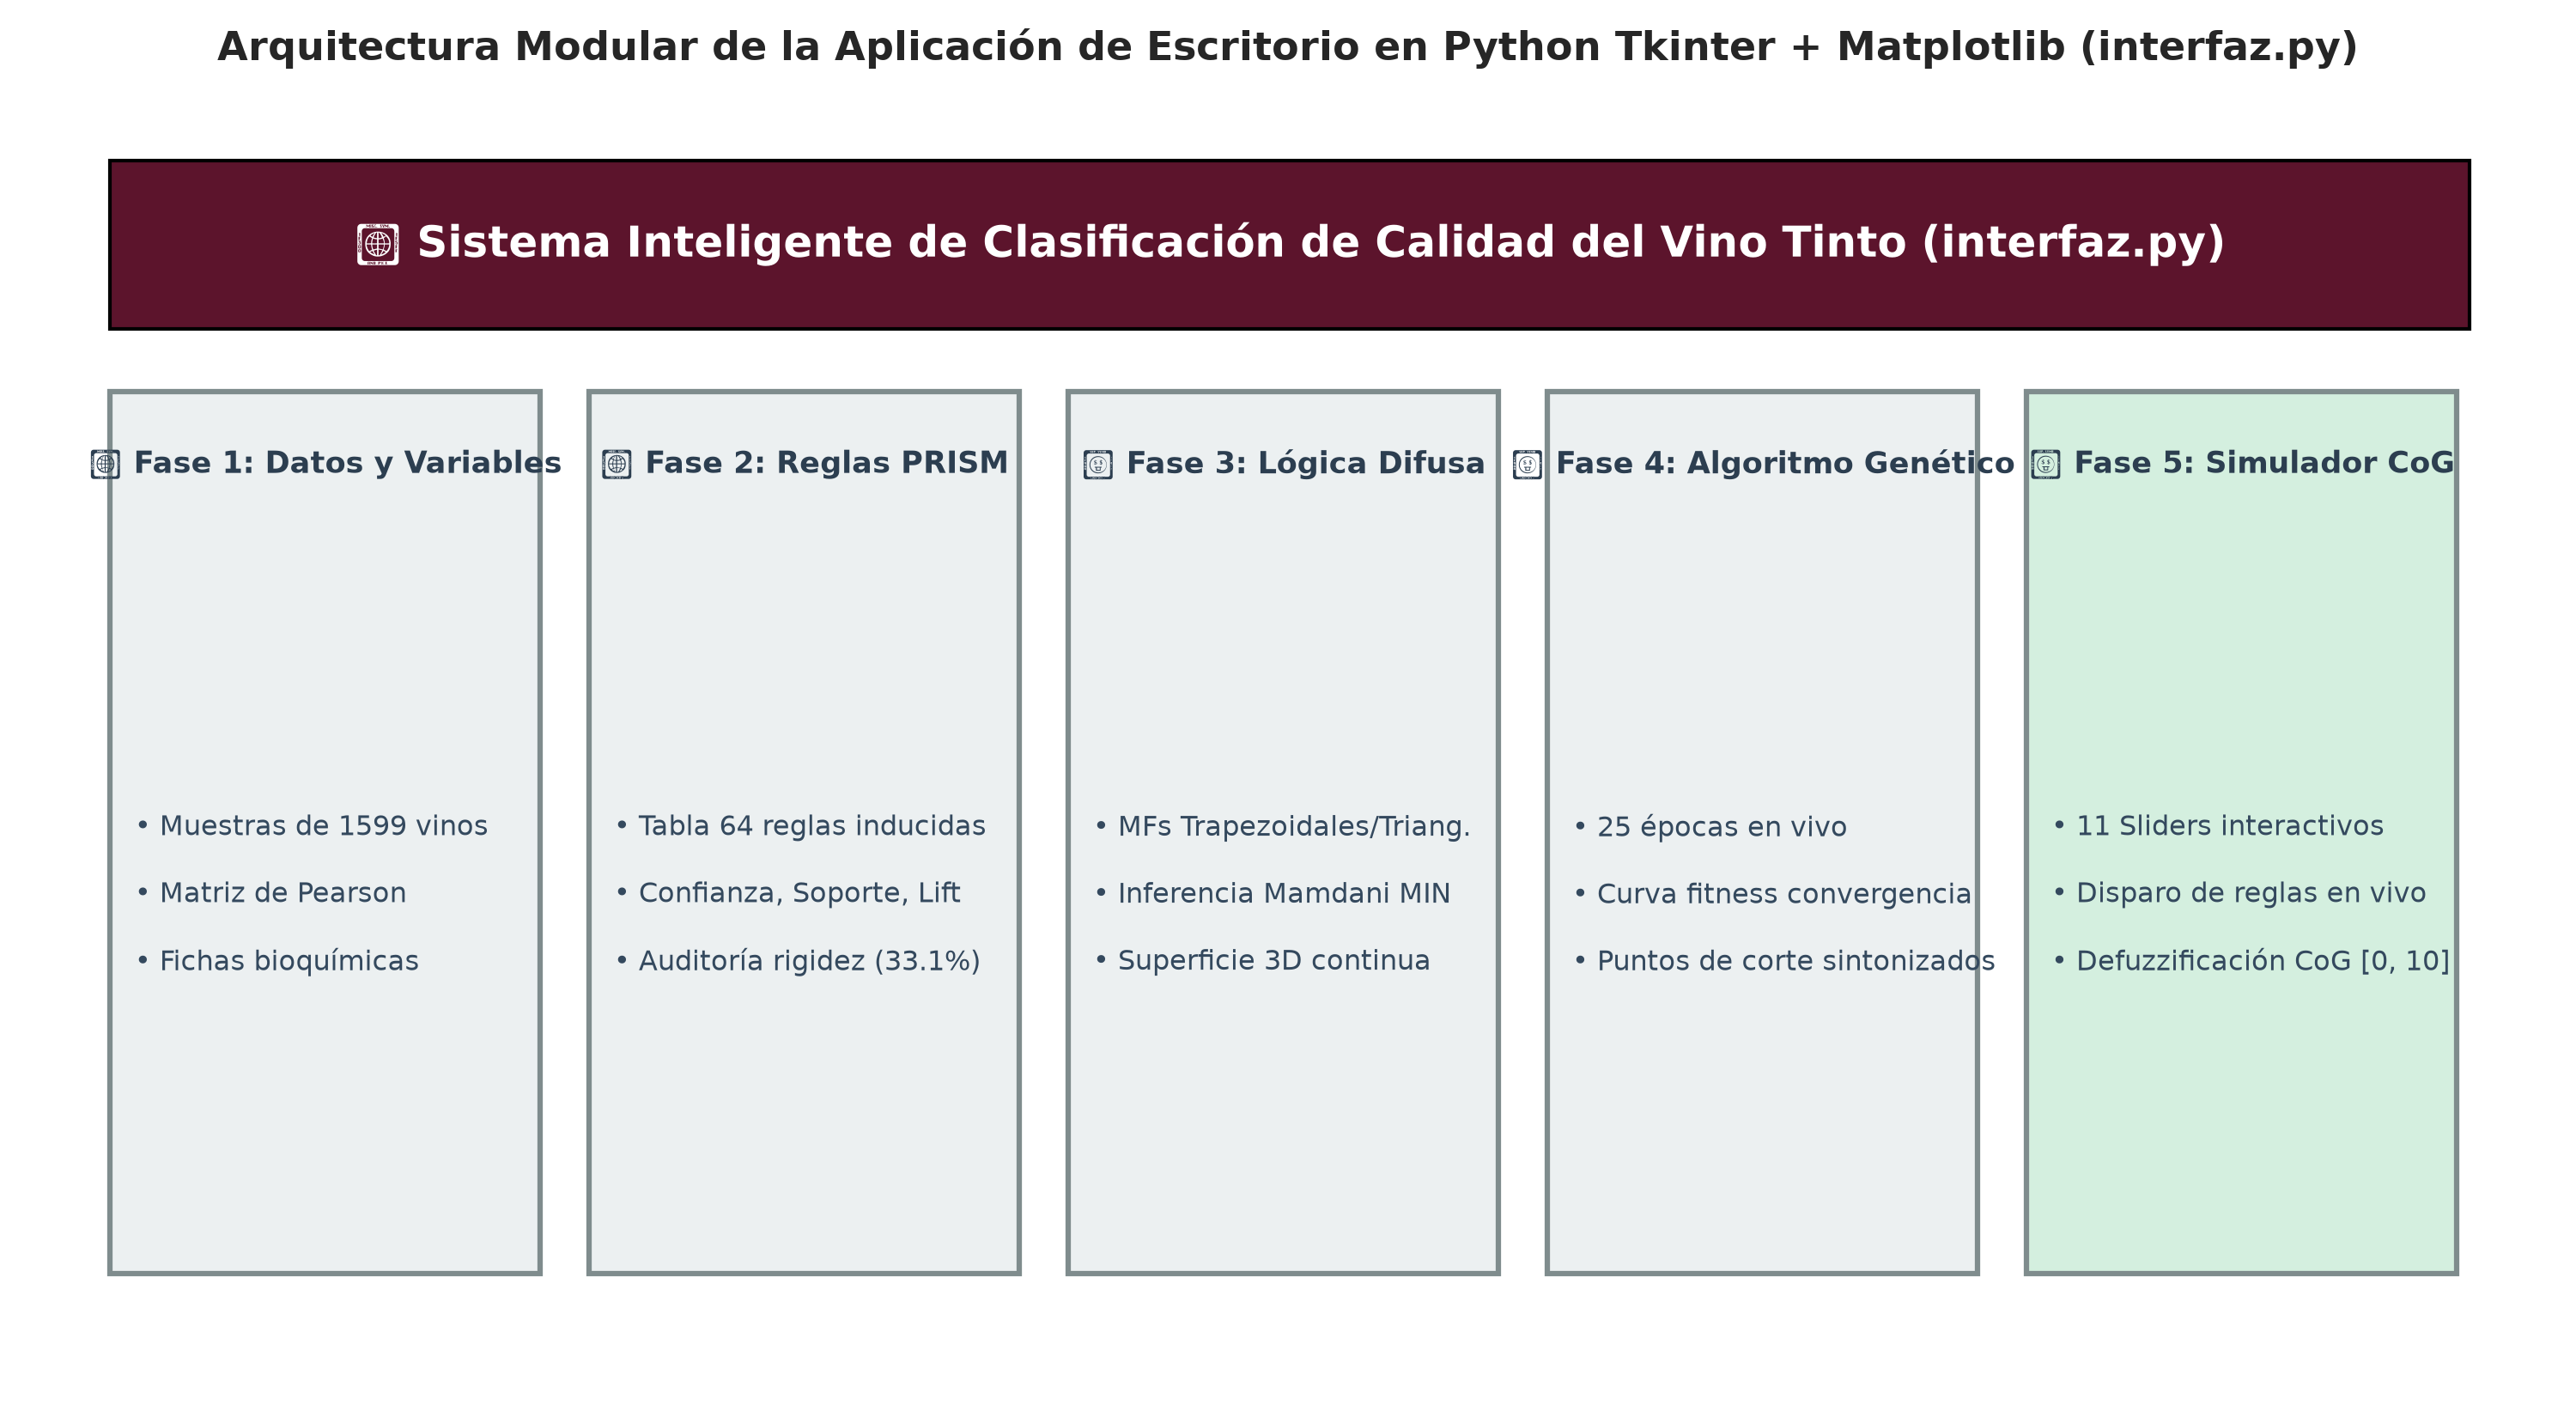
\includegraphics[width=0.95\textwidth]{imagenes/09_interfaz_tkinter_pestanas.png}
\caption{Arquitectura y estructura de navegación de la suite de escritorio en Tkinter (\texttt{interfaz.py}) con sus 5 pestañas de experimentación.}
\label{fig:interfaz_tkinter}
\end{figure}

\begin{enumerate}
    \item \textbf{Pestaña 1 (Fase 1: Datos y Variables):} Despliega una tabla interactiva con las 1,599 instancias fisicoquímicas continuas del dataset \textit{Wine Quality}, cálculo instantáneo de estadísticas descriptivas (media, desviación estándar, cuantiles), matriz de correlación de Pearson y fichas técnicas con la justificación bioquímica de las 11 variables.
    \item \textbf{Pestaña 2 (Fase 2: Reglas PRISM):} Visualizador dinámico de las 64 reglas modulares inducidas con sus métricas formales de minería (Confianza $P(C_j \mid A)$, Soporte, Cobertura y $\text{Lift}$), organizadas por clase consecuente. Incorpora una consola de auditoría booleana rígida que ejecuta la prueba discreta ($N=320$) y evidencia visualmente el colapso del \textit{Boundary Problem} (33.12\% de exactitud con severa abstención).
    \item \textbf{Pestaña 3 (Fase 3: Lógica Difusa Mamdani):} Graficador interactivo de las funciones de pertenencia continuas (curvas trapezoidales y triangulares) y renderizado tridimensional interactivo de la superficie de decisión enológica (e.g., Alcohol vs. Acidez Volátil vs. Calidad CoG), permitiendo rotar la perspectiva en 3D en tiempo real.
    \item \textbf{Pestaña 4 (Fase 4: Algoritmo Genético):} Panel de monitoreo evolutivo en vivo, visualización de la curva de convergencia de aptitud generacional ($25$ épocas en $\approx 15.1\,\text{s}$), histogramas de aptitud poblacional y comparativa morfológica de los puntos de corte difusos pre y post calibración.
    \item \textbf{Pestaña 5 (Fase 5: Clasificador y Defuzzificación CoG en Tiempo Real):} Consola interactiva equipada con controles deslizantes (\textit{sliders}) continuos para las 11 variables fisicoquímicas, activación en vivo de reglas disparadas $\alpha_k$, agregación continua tipo Mamdani mediante la S-norma de máximo y cálculo continuo del Centroide de Gravedad (CoG) con línea vertical directriz sobre el universo $[0, 10]$, emitiendo la clasificación enológica explicable (\textit{Baja}, \textit{Media} o \textit{Alta}).
\end{enumerate}

% =========================================================
% REFERENCIAS BIBLIOGRÁFICAS
% =========================================================

\printbibliography

\end{document}